%%Designed for IEEE Transactions on Vehicular Technology, based on bare_jrnl.tex by Michael Shell.
%%December. 2015
%%Length Requirements: The complete manuscript should be prepared in final IEEE typesetting with maximum page length limited to 15 pages for a Regular Paper and 5 pages  for a Correspondence.
%%Contact Info: admin-tvt@ece.ufl.edu
%%Designed by TVT editorial office


\documentclass[journal,10pt]{IEEEtran}
\usepackage[cmex10]{amsmath}
\usepackage[dvips]{graphicx}
\usepackage{algorithm}
\usepackage{algorithmic}
\usepackage{array}
\usepackage{amssymb}
\usepackage{enumerate}


\newcommand{\PreserveBackslash}[1]{\let\temp=\\#1\let\\=\temp}
\newcolumntype{C}[1]{>{\PreserveBackslash\centering}p{#1}}
\newcolumntype{R}[1]{>{\PreserveBackslash\raggedleft}p{#1}}
\newcolumntype{L}[1]{>{\PreserveBackslash\raggedright}p{#1}}


\begin{document}

\title{Optimal Wireless Energy Redistribution in WSNs}


\author{Author1, Author2, Author3

\thanks{The authors are with the Department of }% <-this % stops a space
\thanks{Manuscript received XXX, XX, 2018; revised XXX, XX, 2018.}}

\markboth{IEEE Transactions on XXX XXX,~Vol.~XX, No.~XX, XXX~2019}
{}
%{Shell \MakeLowercase{\textit{et al.}}: Bare Demo of IEEEtran.cls for Journals}


\maketitle


\begin{abstract}
Wireless energy redistribution based on wireless power transfer technology is a core building block for supporting perpetual wireless sensor networks (WSNs) charged with moving or fixed wireless chargers, and it is especially important for prolong the network normal operation time when WCs could not to charge the network timely. In this paper, we investigated the wireless power transfer based energy redistribution (WPTERD) problem in WSNs, which is to redistribute the energy among network nodes so that all nodes' expected energy amount are satisfied when possible, meanwhile guaranteeing that the energy lost in this process is minimized, and the time length of the redistribution process is minimized. By analyzing some properties of the WPTERD problem, we propose a two-step approach which solves two embedded sub-problems named WPTERD-Egy and WPTERD-Time in turn. The two sub-problems focus exclusively on the optimization in energy and time, respectively. In the first step, based on some interesting properties of the problem, we re-formulate the WPTERD-Egy problem as a linear programming (LP) problem, which returns the optimal energy transmission time lengths of the nodes leading to minimum energy lost. The core work of the WPTERD-Time problem in the second step is to find a minimum makespan schedule of energy transmission time slices. We prove that the WPTERD-Time problem is NP-hard, and propose a Greedy based Energy ReDistribution Scheduling (GERDS) algorithm to solve it. Numerical simulations illustrate the effectiveness and efficiency of GERDS, which return schedules with minimum energy lost and approximately minimum makespan. By exploiting parallel opportunities of energy transmissions, GERDS reduces makespan by about more than 60\% when compared with a schedule without exploiting the parallel energy transmission opportunities.
\end{abstract}


\begin{IEEEkeywords}
wireless energy redistribution problem, wireless power transfer, task scheduling problem, wireless charging, energy harvesting wireless sensor networks.
\end{IEEEkeywords}


\IEEEpeerreviewmaketitle



\section{Introduction}
\label{sec_intro}
\newtheorem{lemma}{\textbf{Lemma}}
\newtheorem{theorem}{\textbf{Theorem}}
\newtheorem{property}{\textbf{P}}
\newtheorem{corollary}{\textbf{Corollary}}
% The very first letter is a 2 line initial drop letter followed
% by the rest of the first word in caps.
%
% form to use if the first word consists of a single letter:
% \IEEEPARstart{A}{demo} file is ....
%
% form to use if you need the single drop letter followed by
% normal text (unknown if ever used by IEEE):
% \IEEEPARstart{A}{}demo file is ....
%
% Some journals put the first two words in caps:
% \IEEEPARstart{T}{his demo} file is ....
%
% Here we have the typical use of a "T" for an initial drop letter
% and "HIS" in caps to complete the first word.

\IEEEPARstart{R}{ecent} breakthroughs in the areas of Wireless Power Transfer(WPT) technology~\cite{Kurs2007, Cannon2009} and rechargeable batteries~\cite{Kang2006} open up a new dimension to prolonging the lifetime of wireless sensor networks (WSNs). WPT is the transmission of electric energy from a power source to a receiver without a conductor. With recent advances in WPT, it is possible to charge sensor nodes in a relative long distance ($>10$m away)\cite{Guo2017}. It has been validated that sensor node could harvest radio power of 6mW from a wireless charger with 4W transmission power over a distance of 12 meters. The received radio power is 20mW and the transition efficiency is 30 percent~\cite{Nintana2012}.

WPT will have a profound impact on the design of WSNs attributed to its obvious advantages, and hence many research efforts have been devoted to exploiting WPT to enhance WSNs~\cite{Xiang2013}-\cite{Madhja2017}. Some works focus on the application of using dedicated fixed or mobile nodes called wireless chargers (WCs) for powering the normal nodes in WSNs using WPT. Due to the limited number of WCs, some nodes may could not obtain power from the WCs directly. This is true even if there are mobile WCs, because that there may be some restrictions on their movement, or the WCs may be fail temporally. Hence, WPT based Energy ReDistribution (WPTERD) is a core building block for supporting perpetual WSNs.

In recent years some research efforts have been devoted on WPTERD-like application, where the nodes exchange energy in peer-to-peer mode when coming into vicinity of each other during moving, so as to make the nodes' remained energy become more balanced. However, the intrinsic broadcasting feature of energy transmitting signals, which means multiple nodes may harvest energy simultaneously from the signal transmitted by a single node, is not exploited, and hence leads to lower energy efficiency.

In this paper, we focus on the WPTERD problem for WSNs: given a WSN with nodes all equipped with wireless power transceivers and limited energy storages containing some known energy, the task is to redistribute the energy in the network among all nodes through WPT, assuring that the energies of the nodes after the redistribution all do not below their energy expectations, meanwhile the energy loss is minimized and the time length (called makespan) of the energy redistribution process is minimized. We solve the WPTERD problem in two steps. In the first step, basing on a proved property resulted from the widely adopted \textit{energy harvesting additive assumption}, the WPTERD problem with only the minimum energy loss objective (named as WPTERD-Egy) is formalized as a Linear Programming (LP) problem, and can thus be solved to obtain the time lengths of the nodes' energy transmission operations. With the results in the first step, the remanent of the WPTERD problem becomes a task scheduling problem of the nodes' energy transmission operation time intervals, denoted as WPTERD-Time. Proving that the WPTERD-Time is NP-hard, we propose a greedy-based heuristic algorithm named Greedy based Energy ReDistribution Scheduling (GERDS), which makes up the second step. Based on solving the WPTERD-Egy with mature LP solvers, the GERDS algorithm returns an approximate optimal schedule with minimum energy loss, quasi-minimum makespan, and thus solve the WPTERD problem completely. Numerical simulations illustrate the effectiveness and efficiency of GERDS, which return schedules with minimum energy loss and approximately minimum makespan. By exploiting parallel opportunities of energy transmissions, GERDS reduces makespan by about 30\% when compared with a schedule without using the parallel opportunities.

Our main contributions in this paper are as follows:

\begin{itemize}
\item{We solve the WPTERD problem completely by dividing it into two sub-problems WPTERD-Egy and WPTERD-Time, and solve the WPTERD problem in two steps which solve the WPTERD-Egy problem and the WPTERD-Time problem, respectively. This approaches exploits the broadcast nature of wireless signals well, and implicitly realizes the multi-hop energy transmission easily.}
\item{For the WPTERD-Egy problem, we prove that its optimal solutions must be disjoint solutions, where energy transmission time intervals of neighboring nodes should not overlap in time line.}
\item{For the WPTERD-time problem, we prove that it is NP-hard, and propose the GERDS algorithm to solve it and thus the WPTERD problem approximately.}
\end{itemize}

The rest of the paper is organized as follows. Related work is discussed in Section~\ref{sec_relwork}. The models of the problem are described in Section~\ref{sec_model}. Analysis results and the method to solve the WPTERD-Egy problem are described in Section \ref{sec_wpter_egy}. In Section~\ref{sec_wpter_time}, the NP-hard property of the WPTERD-Time problem is proved. In Section~\ref{sec_wpter_last}, the DERS algorithm solving the WPTERD problem directly is provided. Simulation results are provided and discussed in Section~\ref{sec_sim}. Finally, we conclude this work in Section~\ref{sec_conclusion}.

\section{Related Work}
\label{sec_relwork}
Existing works using WPT most related to our work fall into two topics: (1) charging WSNs with fixed WCs; (2) energy redistribution among nodes in WSNs.

\subsection{Charging WSNs with fixed WCs}

In \cite{Xiang2013}, focusing on a WSN containing a fixed wireless charger (WC) as the only energy source for the network, the problem of distributing the energy injected from the access point among all nodes through multi-hop WPT was investigated. In the approach there, the energy transfers in the network are modeled and formulated as multi-hop energy flows, and algorithms were proposed.

WSNs with multiple WCs and multi-hop power transfer technique were focused in \cite{Rault2013}. In this work, considering the energy demand of the nodes, the energy loss that occurs during an energy transmission and the energy capacity limits of the WCs, the problem of determining the minimum number of WCs needed for perpetual operation of the WSN was investigated. The approach there solves the problem in two steps. In the first step, for each possible location of the WCs (WCs are assumed to be located at network nodes), a shortest path tree rooted at this location that covers all the nodes is constructed using the Dikjstra's algorithm. Then in the second step, the problem is transformed to a Mixed Integer Linear Programming (MILP) problem making use of the trees constructed in the first step, and the MILP is solved using mature optimization software packages.

The works in \cite{Guo2017,Guo2016} also devoted to WSNs with multiple WCs, but with an emphasis on exploiting the possibility of multiple WCs charging a single node simultaneously. A more complicated energy harvesting model considering the nonlinear superposition charging effect of simultaneously arrived energy signals was proposed there. Basing on this model, the joint charging utilities for all possible set of the WCs are pre-calculated and then be used to solve the concurrent charging scheduling problem (CCSP), whose objective is to find a schedule for the WCs so as to minimize the time spent on providing each sensor node with at least $E$ energy more. The authors showed that CCSP is NP-hard, and proposed a greedy algorithm based on sub-modular set cover problem as well as a genetic algorithm for the CCSP. However, only one-hop WPT is considered in these works.

Multi-hop wireless power transmission is considerably different from multi-hop data transmission. For data, different transmissions are usually different since they convey different data. For energy, however, energy from any source are equivalent, we need not explicitly construct paths and restrict energy flows along a certain graph. In some sense, opportunistic routing in the wireless network routing realm is more suitable for energy transmission. Hence, finding other mechanisms of multi-hop WPT for the wireless charging of WSNs is of importance.

\subsection{Energy Redistribution Among Nodes}

Some series of recent works \cite{Bulut2014,Niko2016,Niko2017,Madhja2016,Madhja2017} focus on a problem similar to our WPTERD problem for mobile social and sensor networks, which consist of human-carried mobile devices. In these works, energy redistribution is realized using peer-to-peer energy exchange, which happens only when nodes coming into vicinity of each other because of the moving of the person carrying the node.

Firstly in \cite{Bulut2014}, the authors investigated the problem of selecting a subset of nodes to charge the rest nodes in the network such that all nodes can continue normal operations without battery depletion. In \cite{Niko2016}, the authors investigated the problem of efficiently reaching an energy balance among network nodes distributively though peer-to-peer energy exchange. The problem was investigated for two different assumptions: loss-less power exchange and lossy power exchange. Three energy exchange protocols were designed, analyzed and evaluated there. Then the problem was extended to the weighted version in \cite{Niko2017}. The uniform balance version and the weighted balance version of the peer-to-peer energy redistribution problem among star-backbone nodes in WSNs were investigated in \cite{Madhja2016} and \cite{Madhja2017}, respectively.

In these works, energy exchange only happens when two nodes coming into vicinity of each other. As a consequence, their analyses and algorithms do not exploit the intrinsic broadcasting nature of wireless signals as well as the capability of WPT's transferring energy over a distance. Ignoring the possibility of multiple nodes simultaneously harvesting energy from a single node's energy transmitting signals inevitably leads to energy in-efficiency.


\section{System Model}
\label{sec_model}
\subsection{Problem Model}

We consider a WSN consisting of $n$ static nodes $U{=}\{u_1, u_2, \ldots, u_n\}$, where node $u_i$ is positioned at $(x(i),y(i),z(i))$. An example network is shown in Fig.\ref{fig_network}. The nodes are equipped with energy storage of capacity limits described as function $e_\text{U}{:}\mathcal{N}(n){\rightarrow}\mathcal{R^{+}}$, \textit{i.e.}, the capacity limit of node $u_i$ is $e_\text{U}(i)$. We assume node $u_i$'s energy should always do not below its lower limit $e_\text{L}(i)$. Besides the traditional wireless transmitter/receivers (transceivers) for data communication, these nodes are all equipped with wireless energy transceivers dedicated for transmitting/harvesting energy. Suppose node $u_i$ currently has energy $e_\text{B}(i)$, $i{\in}\mathcal{N}(n)$. We are required to redistribute the energy among the nodes in by using WPT, with the objective that node $u_i$'s energy $e_\text{F}(i)$ at the finish of the redistribution process should not below its expectation $e_\text{E}(i)$, $i{\in}\mathcal{N}(n)$. We express the objective as $e_\text{F}{\succeq}e_\text{E}$ for short. We assume that the energy expectation of node $u_i$ has a lower limit $e_\text{E,L}(i)$. We also assume $e_\text{L}{\prec}e_\text{E,L}{\preceq}e_\text{E}{\prec}e_\text{U}$ and $e_\text{L}{\prec}e_\text{B}{\prec}e_\text{U}$ always hold. For convenient, function $e_\text{U}$ is sometimes called as list or vector when causing no confusion, which also applies to other similar symbols. For easy reference, we list the symbols and their meanings in Table \ref{T1}.

\begin{table}[!htbp]
\centering
\caption{Notations and meanings.}
\label{T1}
\footnotesize{
\begin{tabular}
{|p{0.05\textwidth}|p{0.38\textwidth}|}
\hline
\textbf{Notation} & Meaning\\
\hline
$\mathcal{N}(n)$ & The set of positive integers $\{1,2,\ldots,n\}$;\\
\hline
$\mathcal{R^{+}}$ & The set of positive real value in range $[0,{+}\inf]$;\\
\hline
$p, \mathbf{p}$ & The function/list/vector of the node's constant energy transmitting power, node $u_i$'s energy transmit power is $p(i)$;\\
\hline
$[.]^{\text{T}}$ & Transpose operation of the input matrix or vector;\\
\hline
$\mathbf{C}$ & The matrix of the energy harvesting coefficients $[c(i,j]_{i,j{\in}\mathcal{N}(n)}$, c(i,j) is the energy harvesting coefficient for node $u_i$ receives energy from $u_j$;\\
\hline
$\mathbf{t}$ & The vector of the nodes' energy transmitting time lengths $\mathbf{t}{\triangleq}[t(1),t(2),\ldots,t(n)]^{\text{T}}$;\\
\hline
$e_\text{B}, \mathbf{e_\text{B}}$ & The function/list/vector of the nodes' energy at the beginning time where it is $e_\text{B}(i)$ for $u_i$.  $\mathbf{e_\text{B}}{\triangleq}[e_\text{B}(1),e_\text{B}(2),\ldots,e_\text{B}(n)]^{\text{T}}$;\\
\hline
$e_\text{F}, \mathbf{e_\text{F}}$ & The function/list/vector of the nodes' final energy after the energy redistribution process finishes where it is $e_\text{F}(i)$ for $u_i$. $\mathbf{e_\text{F}}{\triangleq}[e_\text{F}(1),e_\text{F}(2),\ldots,e_\text{F}(n)]^{\text{T}}$;\\
\hline
$e_\text{U}, \mathbf{e_\text{U}}$ & The function/list/vector of the nodes' energy upper limits where it is $e_\text{U}(i)$ for $u_i$. $\mathbf{e_\text{U}}{\triangleq}[e_\text{U}(1),e_\text{U}(2),\ldots,e_\text{U}(n)]^{\text{T}}$;\\
\hline
$e_\text{L}, \mathbf{e_\text{L}}$ & The function/list/vector of the nodes' energy lower limits where it is $e_\text{L}(i)$ for $u_i$. $\mathbf{e_\text{L}}{\triangleq}[e_\text{L}(1),e_\text{L}(2),\ldots,e_\text{L}(n)]^{\text{T}}$;\\
\hline
$e_\text{E}, \mathbf{e_\text{E}}$ & The function/list/vector of the nodes' energy expectations where it is $e_\text{E}(i)$ for $u_i$. $\mathbf{e_\text{E}}{\triangleq}[e_\text{E}(1),e_\text{E}(2),\ldots,e_\text{E}(n)]^{\text{T}}$;\\
\hline
$e_\text{E,L}, \mathbf{e_\text{E,L}}$ & The function/list/vector of the nodes' lower limits of energy expectations where it is $e_\text{E,L}(i)$ for $u_i$. $\mathbf{e_\text{E,L}}{\triangleq}[e_\text{E,L}(1),e_\text{E,L}(2),\ldots,e_\text{E,L}(n)]^{\text{T}}$;\\
\hline
$\mathbf{1}$ or $\mathbf{0}$ & Proper size column vectors with elements all one or all zero, respectively;\\
\hline
$\mathbf{1}_{condi}$ & The indication function of condition $condi$, which has value 1 when $condi$ is true, and 0 otherwise;\\
\hline
$N(i)$ & The set of neighbors of node $u_i$, two nodes $u_i$ and $u_j$ are neighbors of each other if $c(i,j){+}c(j,i){>}0$ ;\\
\hline
$N_{H,\text{y}}(v)/N_{H,\text{n}}(v)$ & The set of node $v$'s neighbors in graph $H$ together with/without node $v$ itself;\\
\hline
$w(S)$ & The accumulated weight of the nodes in S;\\
\hline
$\varpi(G)$ & $\varpi(G){\triangleq}\max_{H{\subseteq}G}(\min_{v{\in}H}w(N_{H,\text{y}}(v))$;\\
\hline
\end{tabular}
}
\end{table}

\begin{figure}[htb]
\centering{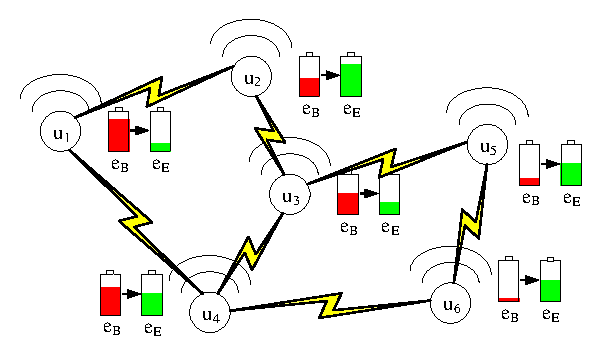
\includegraphics[width=0.48\textwidth]{fig1_network.eps}}
\caption{An example network with WPT based energy redistribution.}
\label{fig_network}
\end{figure}

Assume node $u_i$ always transmits energy with a constant power $p(i)$, $i{\in}\mathcal{N}(n)$. When node $u_i$ is transmitting energy, the energy power harvested by node $u_j$ from $u_i$'s signal is expressed as $p_\text{H}(j){=}c(j,i){*}p(i)$, where the energy harvesting coefficient $c(i,j)$ abstracts the effects of many factors such as the distance between the nodes, the environment, the hardware restriction, etc. Energy harvesting coefficients are always non-negative. If $c(i,j){+}c(j,i){>}0$, then we say that $u_i$ and $u_j$ are neighbors. Furthermore, because of the energy conservation principle in practice, energy loss is inevitable during the wireless energy redistribution process, hence we assume $\sum_{j{\neq}i,j{\in}\mathcal{N}(n)}c(j,i){<}1$, $i{\in}\mathcal{N}(n)$. For completeness, we let $c(i,i){=}{-}1$, $i{\in}\mathcal{N}(n)$. We collect all energy harvesting coefficients into a matrix $\mathbf{C}{=}[c(i,j)]_{i,j{\in}\mathcal{N}(n)}$.

We assume that the energy harvesting coefficients of the nodes are constant. Moreover, multiple simultaneous energy transmissions encountered at a node are assumed to be additive, which is the \textit{energy harvesting additive assumption} widely adopted in the literature\cite{He2013,Dai2017TON,Dai2018TON}. In other words, if a set of nodes $\{u_j|j{\in}U_\text{s}\}$ transmit energy with power $\{p_j|j{\in}U_\text{s}\}$ to another node $u_j$ simultaneously, then the energy power harvested by $u_j$ is $p_\text{H}(j){=}\sum_{k{\in}U_\text{s}}c(j,k){*}p(k)$. Harvested energy should be stored in the energy storage for later use. Excessive energy harvested by node $u_i$ is lost when the energy storage is full of energy.

To fulfil the objective of the WPTERD problem, we have to find an energy transmission schedule $s_\text{c}{\triangleq}\{s(1),s(2),\ldots\}$ where $s(i){\triangleq}(u_\text{s}(i), t_\text{b}(i),t_\text{e}(i))$ represents a schedule item, which means to let node $u_\text{s}(i){\in}U$ transmit energy in time slice $[t_\text{b}(i),t_\text{e}(i)]$. Given a schedule, if each node $u_i$ can only exist in at most one schedule item, then this schedule is \textit{non-preemptive}, otherwise it is \textit{preemptive}. We mainly consider preemptive schedules in this paper. An energy transmission schedule is valid if we have $e_\text{F}{\succeq}e_\text{E}$ after performing the energy redistribution process according to the schedule. A valid schedule with \textit{maximum accumulated final energy} $E_\text{C}(s_\text{c}){=}\sum_{i{=}1}^{n}e_\text{F}(i)$ is called an \textit{optimal schedule}. For the WPTERD problem, it is obvious that \textit{maximizing accumulated final energy} is equivalent to \textit{minimizing the energy loss}, hence we use the two phases alternatively for convenience. We denote $t_\text{E}(s_\text{c}){\triangleq}\max_{i{:}s(i){\in}s_\text{c}}t_\text{e}(i)$ and call it the \textit{schedule length} of $s_\text{c}$. Short schedules are preferred. In the literature of job/task scheduling, it has the \textit{makespan}~\cite{Marx2004}. We will use the two concepts alternatively for convenience.

\textbf{Formally, we state our WPTERD problem as follows}. \textit{Given a set of static nodes $U$ in a given space with energy harvesting coefficient matrix $C{=}\{c(i,j)\}$, energy storage capacity limit list $e_\text{U}$ (vector), energy storage lower limit list $e_\text{L}$, energy transmitting power list $p$, beginning energy list $e_\text{B}$, expected energy list $e_\text{E}$, the task is to find a valid energy transmission schedule $s_\text{c}$ with maximum accumulated final energy $E_\text{C}(s_\text{c})$ and further with minimum makespan $t_\text{E}(s_\text{c})$}.


\subsection{Energy Harvesting Model}

The energy harvesting model determines the energy harvesting coefficients. Although any energy harvesting model can be applied, we adopt a model where energy harvesting coefficient is determined using Eq.\eqref{eqn_model_charge}. In \eqref{eqn_model_charge}, $\alpha$,$\beta$,$\gamma$ are known constants determined by hardware parameters of the energy transceivers as well as the surrounding environment, and $D$ is the farthest distance that the energy transmitting signal can reach when the energy transmitting power $p{=}1$. $\gamma{\in}[2,6]$ represents the channel fading effect and it is 4 in free space.

\begin{equation}
\label{eqn_model_charge}
c(d){=}\left\{
\begin{array}{ll}
\frac{\alpha}{(\beta{+}d)^{\gamma}}, \hspace{3mm}&d{\leq}D{*}p^{1/\gamma};\\
0,&d{>}D{*}p^{1/\gamma},
\end{array}
\right.
\end{equation}

Our energy harvesting model extends the model in \cite{Dai2017TON} in two aspects: (1) adds one new parameter $\gamma$, which consists with the popular wireless signal transmission model; (2) makes the energy coverage radius depends on the energy transmitting power, which is more practical. Furthermore, the model is not restricted to 2D or 1D space, in fact 3D space also applies.

Comment: \textit{the analyses and proposed algorithm in later sections do not depend on certain energy harvesting model. The model in \eqref{eqn_model_charge} is only used in the simulation experiments in Section~\ref{sec_sim}}.

\section{Solve the WPTER-Egy Problem}
\label{sec_wpter_egy}

By analyzing some properties of the WPTERD problem, we propose a two-step approach which solves two embedded sub-problems named WPTERD-Egy and WPTERD-Time in turn. The two sub-problems focus only on the optimization in energy and time, respectively. In the first step, by formulating the WPTERD-Egy problem based on interesting property of the problem in a linear programming (LP) form, we obtain the optimal energy transmitting time lengths of the nodes leading to minimum energy loss. With the results in the first step, the remanent work of the WPTERD problem becomes the WPTERD-Time problem, which is to find a minimum makespan schedule of energy transmission operations not violating the nodes' energy limits. We call a continuous time interval of a node's energy transmission operation as an \textit{energy transmission time slice}, hence the WPTERD-Time problem is to schedule the energy transmission time slices. We use \textit{time slice} to represent \textit{energy transmission time slice} by default for simplicity.

We will provide our analysis and treatment on the WPTERD-Egy problem in this section. The treatments on the WPTERD-Time problem are provided in later sections.

\subsection{Problem Formulation of the WPTERD-Egy Problem}

Let $S_\text{C}$ be the space of all valid energy transmission schedules. Given a schedule $s_\text{c}{\in}S_\text{C}$, we can sort all items of $t_\text{b}(i)$ and $t_\text{e}(i)$ into a list $T_\text{s}(s_\text{c}){=}[t_1,t_2,\ldots,t_{L}]$ in ascending order. Here the list is assumed to have length $L$. The time points in $T_\text{s}(s_\text{c})$ divide the time interval $[0,t_\text{L}]$ into time slots $\{ts(1),ts(2),\ldots,ts(n)\}$, where $ts(i)$ represents the slot $(t_{i{-}1},t_i]$. For each slot $ts(i)$, we can obtain the set of nodes $U_\text{T}(i)$ who are scheduled to transmit energy in slot $ts(i)$, and meanwhile all the others $U_\text{H}(i){=}U{-}U_\text{T}(i)$ harvest energy.

During the energy redistribution process, node $u_i$'s energy changes along time $t{\in}[0,t_{L}]$. Denoting the function of $u_i$'s energy on time $t$ and energy transmission schedule $s_\text{c}$ as $e_i(s_\text{c},t)$, then it can be expressed recursively as Eq.\eqref{eqn_energyfun_time}.

\begin{figure*}
\begin{equation}
\label{eqn_energyfun_time}
e_i(s_\text{c},t){=}\left\{
\begin{array}{ll}
e_\text{B}(i), \hspace{3mm}&t{=}0;\\
\min\left\{e_\text{U}(i),
\max\left[0,
e_i(s_\text{c},t_{j{-}1})
{+}\left(
\mathbf{1}_{i{\in}U_\text{H}(j)}
\mathop{\sum}\limits_{k{\in}U_\text{T}(j)}p(k)c(k,i)
{-}
\mathbf{1}_{i{\in}U_\text{T}(j)}p(i)
\right)
(t{-}t_{j{-}1})
\right]
\right\}
,&t{\in}(t_{j{-}1},t_j],\\
&j{\in}\mathcal{N}(L);
\end{array}
\right.
\end{equation}
\end{figure*}

The WPTERD-Egy problem can then be formulated as Eq.\eqref{eqn_wpterd_egy}.

\begin{equation}
\label{eqn_wpterd_egy}
\begin{array}{rcl}
(\textbf{P1})&\mathop{\max}\limits_{s_\text{c}{\in}S_\text{C}}&{\sum}_{u_i{\in}U}e_i(s_\text{c},t_\text{E}(s_\text{c}))\\
&\textit{s.t.}&e_i(s_\text{c},t_E(s_\text{c})){\geq}e_\text{E}(i),\hspace{3mm}i{\in}\mathcal{N}(n);\\
&&e_i(s_\text{c},t_\text{E}(s_\text{c})){\leq}e_\text{U}(i),\hspace{3mm}i{\in}\mathcal{N}(n);\\
&&e_i(s_\text{c},t){\leq}e_\text{U}(i),\hspace{3mm}i{\in}\mathcal{N}(n),t{\in}[0,t_\text{E}(s_\text{c})];\\
&&e_i(s_\text{c},t){\geq}e_\text{L}(i),\hspace{3mm}i{\in}\mathcal{N}(n),t{\in}[0,t_\text{E}(s_\text{c})];
\end{array}
\end{equation}

The WPTERD-Egy problem has several challenges: (1) it is nonlinear due to the lower and upper limits of nodes energy; (2) the solution space $S_\text{C}$ is infinitely larger because that the variables $t_i$ can take any real values from the continuous time interval $[0, t_\text{E}(s_\text{c})]$, and $t_\text{E}(s_\text{c})$ also requires to be determined.

Further inspections show that, what significantly affect the nodes' final energy are their energy transmission time lengths, not the beginning and ending time of the time slots. Hence, to overcome the challenges, we will focus only on determining the optimal energy transmission time lengths leading to minimum energy loss in the WPTERD-Egy problem.

\textit{The restrictions on each node's energy of not violating the lower and upper energy limits during the energy redistribution process are postponed to the WPTERD-Time problem, and hence are ignored in the WPTERD-Egy problem}.

\subsection{Analyses on the WPTERD-Egy Problem}
During the energy redistribution process, excessive energy harvested of a node is lost when its energy storage is full of energy. Given an energy transmission schedule, if some harvested energy are lost at some nodes, we say that \textit{this schedule has energy upper limit violations}.

About energy transmission schedules with energy upper limit violations, we have the following lemma.
\begin{lemma}
\label{lemma_violation}
For any valid energy transmission schedule with some energy upper limit violations, there must be some valid energy transmission schedules with more accumulated final energy.
\end{lemma}

\begin{IEEEproof}
Without loss of generality, we denote the given schedule with violations as $s_0$, and assume the violation is happened at node $v_0{\in}U$. Then we analyze the situation by dividing into the following two cases:
\begin{itemize}
\item{\textbf{case1: ${\exists}v_i{\in}N(v_0)$ with $e_\text{F}(v_i){<}e_\text{U}(v_i)$}}.
For the purpose to generate a better schedule with no violation, we assume each node is equipped with an auxiliary energy storage which can store the lost energy because of the violation on its energy upper limits. Then, after $s_0$ finishes, we can let node $v_0$ try to use-up the energy in its auxiliary storage (assume the amount of the energy is $e_{v0}$) by an additional energy transmission time slice of length $e_{v0}/p(v_0)$. The node $v_i$ will harvest energy $c(v_i,v_0){*}p(v_0)*{e_{v0}{/}p(v_0)}{=}c(v_i,v_0){*}e(v_0)$ from this energy transmission, and its new final energy will becomes $e'_\text{F}(v_i){=}\max(e_\text{F}(v_i){+}c(v_i,v_0){*}e(v_0),e_\text{U}(v_i))$. With the given condition that $e_\text{F}(v_i){<}e_\text{U}(v_i)$, we have $e'_\text{F}(v_i){>}e_\text{F}(v_i)$. Meanwhile, all other nodes' new final energy will at least not decrease. Thus, total accumulated final energy after $v_0$'s last energy transmission will be greater than that of $s_0$. Furthermore, we can obtain a new schedule $s_1$ by scheduling $v_0$'s last energy transmission to earlier times such that the violation at $v_0$ does not happens, which is true since that we can extend the makespan of the whole schedule when necessary. The new schedule $s_1$ may still have violations at other nodes, but the violation at node $v_0$ is avoided.

\item{\textbf{case2: ${\forall}v_i{\in}N(v_0)$ we have $e_\text{F}(v_i){=}e_\text{U}(v_i)$}}.
In this case, there must be a node $v_1$ with $e_F(v_1){<}e_\text{U}(v_1)$ in the network such that there is a path $\{v_0{=}a_1,a_2,\ldots,a_k{=}v_1\}$ connects $v_0$ and $v_1$, as illustrated in Fig.\ref{fig_path}. As in the previous case, we also assume each node is equipped with an auxiliary energy storage. Then, after $s_0$ finishes, we can let node $a_i$,$i{\in}\mathcal{N}(k{-}1)$, to make additional energy transmissions in turn so as to use-up the excessive energy $e_{v0}$ at $v_0$, meanwhile make $e'_\text{F}(a_i){=}e_\text{F}(a_i){=}e_\text{U}(v_i)$, $i{\in}\mathcal{N}(k{-}1)$, $e'_\text{F}(a_k){>}e_\text{F}(a_k)$. The time lengths of the additional transmissions $t(a_i)$, $i{\in}\mathcal{N}(k{-}1)$, can be obtained by solving the following Eq.\eqref{eqn_violation_proof}. Furthermore, we can obtain a new schedule $s_1$ by scheduling these additional energy transmissions to earlier times such that violations at $a_i$, $i{\in}\mathcal{N}(k{-}1)$, do not happen.

\begin{figure*}
\begin{equation}
\label{eqn_violation_proof}
\left[
\begin{array}{c c c c c}
-1{*}p(a_1)          &   c(a_1,a_2){*}p(a_2)  &          \ldots    & 0      &   0\\
c(a_2,a_1){*}p(a_1)  &       -1{*}p(a_2)      &    \ldots    & 0      &    0\\
    0       &   c(a_3,a_2){*}p(a_2)         &    \ldots  & 0      &   0\\
    0       &   0           &         \ddots     &-1{*}p(a_{k{-}2})      &c(a_{k{-}2},a_{k{-}1}){*}p(a_{k{-}1})\\
    0       &   0           &            0    & c(a_{k{-}1},a_{k{-}2}){*}p(a_{k{-}2})     & -1{*}p(a_{k{-}1})\\
\end{array}
\right]
\left[
\begin{array}{c}
t(a_1)\\
t(a_2)\\
\vdots\\
t(a_{k{-}2})\\
t(a_{k{-}1}\\
\end{array}
\right]
{=}
\left[
\begin{array}{c}
-e_{v0}\\
0\\
0\\
\vdots\\
0\\
\end{array}
\right]
\end{equation}
\end{figure*}

\end{itemize}

Combining above cases, the lemma follows.
\end{IEEEproof}

\begin{figure}[htb]
\centering{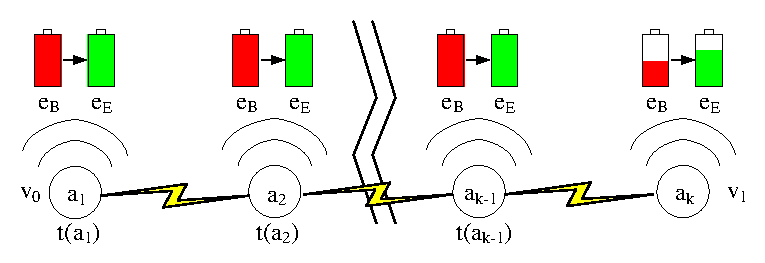
\includegraphics[width=0.48\textwidth]{fig2_path.eps}}
\caption{The path connects $v_0$ and $v_1$ with $e_\text{F}(v_1){<}e_\text{U}(v_1)$.}
\label{fig_path}
\end{figure}


Based on Lemma~\ref{lemma_violation}, we have the following theorem further.

\begin{theorem}
\label{theorem_no_violation}
Optimal energy transmission schedules with maximum accumulated final energy (\textit{i.e.}, minimum energy loss) must have no upper limit violations.
\end{theorem}

\begin{IEEEproof}
It can be proved easily by contradiction. If there is an optimal schedule $s_1$ with violations, then by applying Lemma~\ref{lemma_violation} we can obtain a new better schedule $s_2$, which contradicts with the assumption that $s_1$ is optimal.
\end{IEEEproof}


\textit{For any energy transmission schedule $s_1$, if there is a set of neighboring nodes whose time slices in $s_{1}$ overlap(partly or completely), then we can obtain a new schedule $s_{2}$ by just moving the overlapped time slices apart meanwhile guaranteeing that they all do not overlap with all other nodes' time slices}. This is absolutely possible since that we can always increase $t_L$ when necessary. We call a schedule where neighboring nodes' time slices do not overlap as a \textit{disjoint schedule}, otherwise an \textit{overlap schedule}.

For the relative priority of the two schedules $s_1$ and $s_2$ in term of accumulated final energy $E_\text{C}$, we have the following lemma.

\begin{lemma}
\label{lemma_interval_disjoint}
For the two energy transmission schedules $s_1$ and $s_2$ obtained as above and assume they both have no energy upper limit violations, we have $E_\text{C}(s_2){>}E_\text{C}(s_1)$.
\end{lemma}

\begin{IEEEproof}
Basing on the \textit{energy harvesting additive assumption}, and according to Eq.\eqref{eqn_energyfun_time}, we analyze the following cases:
\begin{itemize}
\item{\textbf{case1: the set of neighboring nodes whose time slices overlap only contains two nodes}}.

Assume the two neighboring nodes as $u_i$ and $u_j$. Replacing $s_1$ with $s_2$ will not affect the amount of energy harvested by any other node $u_k$, \textit{i.e.}, $e_k(s_1,t_\text{E}(s_1)){=}e_k(s_2,t_\text{E}(s_2))$, ${\forall}k{\in}\mathcal{N}(n), k{\neq}i,j$. It is also easy to notice that, the energy harvested by $u_i$ and $u_j$ from all the other nodes are kept unchanged when replacing $s_1$ with $s_2$.

Now we analyze the harvested energy of $u_i$ from $u_j$ in $s_1$ and $s_2$, respectively. We assume the lengths of $u_i$ and $u_j$'s energy transmitting time intervals in $s_1$ are respectively $t(i)$ and $t(j)$. Furthermore, assume that the total length of overlapped parts of their time slices has length $t_\text{o}$. Thus, the energy harvested by $u_i$ from $u_j$ in $s_1$ is $c_{i,j}{*}p(j){*}(t(j){-}t_\text{o})$. Contrastively, since that the time slices of $u_i$ and $u_j$ in $s_2$ are disjoint, the energy harvested by $u_i$ from $u_j$ in $s_2$ becomes $c_{i,j}{*}p(j){*}t(j)$. Since that $c(i,j){\geq}0$, $u_i$'s final energy $e_i(s_2,t_\text{E}(s_2)){\geq}e_i(s_1,t_\text{E}(s_1))$. The same analysis applies to $u_j$ and we have $e_j(s_2,t_\text{E}(s_2)){\geq}e_j(s_1,t_E(s_1))$. With the fact $c_{i,j}{+}c_{j,i}{>}0$ for neighboring nodes $u_i$ and $u_j$, we know that at least one $e_k(s_2,t_\text{E}(s_2)){\geq}e_k(s_1,t_\text{E}(s_1))$, $k{\in}\{i,j\}$, strictly holds. Considering the given pre-condition that there are no energy upper limit violations, all harvested energy will be able to be stored, hence we have Eq.\eqref{eqn_disjoint_proof}.

\begin{equation}
\label{eqn_disjoint_proof}
\begin{array}{rl}
E_\text{C}(s_2)&{=}e_i(s_2,t_\text{E}(s_2)){+}e_j(s_2,t_\text{E}(s_2)\\
&\hspace{3mm}
{+}\mathop{\sum}_{{k{\in}\mathcal{N}(n),k{\neq}i,j}}e_k(s_2,t_\text{E}(s_2)\\
&{>}e_i(s_1,t_\text{E}(s_1)){+}e_j(s_1,t_E(s_1)))\\
&\hspace{3mm}
{+}\mathop{\sum}_{{k{\in}\mathcal{N}(n),k{\neq}i,j}}e_k(s_1,t_\text{E}(s_1))\\
&{=}E_\text{C}(s_1).
\end{array}
\end{equation}


\item{\textbf{case2: the set of neighboring nodes whose time slices overlap contains three or more nodes}}.
Without loss of generality, we assume the set contains $k$ nodes $U_\text{s}{=}\{u_{s1},u_{s2},\ldots,u_{sk}\}$. Following the same way as in case1, we can analyze the energy of each node in $U_\text{s}$ harvested from the other nodes in $U_s$. We can thus obtain that each node's harvested energy in $s_2$ must be greater than that in $s_1$. Again with the fact that there are no energy upper limit violations, we have $E_\text{C}(s_2){>}E_\text{C}(s_1)$.

\end{itemize}

Combining above cases, the lemma follows.
\end{IEEEproof}

By combining the previous Theorem~\ref{theorem_no_violation} and Lemma~\ref{lemma_interval_disjoint}, we can obtain the following theorem easily.

\begin{theorem}
\label{theorem_schedule_disjoint}
Optimal energy transmission schedules with maximum accumulated final energy (\textit{i.e.}, minimum energy loss) must be disjoint.
\end{theorem}

\begin{IEEEproof}
We prove it by contradiction. Assume there is an optimal solution $s_1$ which is not disjoint. By Theorem~\ref{theorem_no_violation}, we know that $s_1$ must have no violations. Then by using Lemma~\ref{lemma_interval_disjoint} on $s_1$, we can obtain a better schedule $s_2$, which contradicts with the assumption that $s_1$ is optimal.
\end{IEEEproof}

\subsection{Reformulate and Solve the WPTERD-Egy Problem}

Theorem~\ref{theorem_schedule_disjoint} tells us that, to solve the WPTERD-Egy problem, we need only to consider disjoint schedules, which enables us to re-formulate the WPTERD-Egy problem as a more simplified linear programming (LP) problem and thus easy to solve.

Let $t_i$ be the total length of node $u_i$'s energy transmission time slices (called as time length of $u_i$ for short) in a schedule, and let $t{\triangleq}\{t(1),t(2),\ldots,t(n)\}$ be the list of all nodes' time lengths, then the final energy of node $u_i$ after performing the schedule can be expressed as Eq.\eqref{eqn_final_energy}. Since that we postpone the treatment for not exceeding the energy storage limits when solving the WPTERD-Time problem, we only consider the restriction of the energy limits on the final energy $e_\text{F}$ here.

\begin{equation}
\label{eqn_final_energy}
\begin{array}{rl}
e_\text{F}(i){=}e_\text{B}(i){-}p(i)t_i
{+}&\mathop{\sum}\limits_{\substack{j{\in}\mathcal{N}(n),j{\neq}i}}
c(i,j)p(j)t_j,i{\in}\mathcal{N}(n).\\
\end{array}
\end{equation}

The WPTERD-Egy problem for determining $\mathbf{t}$ can then be expressed as \textbf{P2} in Eq.\eqref{eqn_p2}.

\begin{equation}
\label{eqn_p2}
\begin{array}{rcll}
(\textbf{P2})&\mathop{\max}\limits_{t{=}\{t(1),t(2),\ldots,t(n)\}}&{\sum}_{i{\in}\mathcal{N}(n)}e_\text{F}(i)\\
&\textit{s.t.}
&Eq.\eqref{eqn_final_energy};&\\
&&e_\text{F}(i){\geq}e_\text{E}(i),&i{\in}\mathcal{N}(n);\\
&&e_\text{F}(i){\leq}e_\text{U}(i),&i{\in}\mathcal{N}(n);\\
&&t_i{\geq}0,&i{\in}\mathcal{N}(n).
\end{array}
\end{equation}

Using the matrix and vector symbols defined in Table \ref{T1}, problem \textbf{P2} can be expressed in matrix form as \textbf{P3} in Eq.\eqref{eqn_p3}.

\begin{equation}
\label{eqn_p3}
\begin{array}{rcl}
(\textbf{P3})&\mathop{\max}\limits_{\mathbf{t}}&\mathbf{1}^\text{T}{*}\mathbf{e_\text{F}}\\
&\textit{s.t.}
&\mathbf{e_\text{B}}{+}\mathbf{C}{*}\mathbf{p}{*}\mathbf{1}^{\text{T}}{*}\mathbf{t}{=}\mathbf{e_\text{F}};\\
&&\mathbf{e_\text{F}}{\succeq}\mathbf{e_\text{E}};\\
&&\mathbf{e_\text{F}}{\preceq}\mathbf{e_\text{U}};\\
&&\mathbf{t}{\succeq}0.
\end{array}
\end{equation}

Problem \textbf{P2} (\textit{i.e.}, \textbf{P3}) is a standard linear programming problem, which can be solved efficiently using mature software optimization packages, such as Gurobi, Cplex, Nlopt, and Snopt, Knitro, Conopt, Stoaminlp, Minlpsolve.

\section{Analyses on the WPTERD-Time Problem}
\label{sec_wpter_time}
Given an energy transmission schedule, we can group the schedule items into item sets $S^{i}{=}\{s^{i}_1, s^{i}_2, \ldots, s^{i}_{mi}\}$, $i{\in}\mathcal{N}(n)$. Thus, $S^{i}$ contains all $mi$ schedule items where node $u_i$ should transmit energy. Thus, the total energy transmission time length of $u_i$ contains $mi$ time slices with length $t_\text{e}(s^{i}_j){-}t_\text{b}(s^{i}_j)$, $j{\in}\mathcal{N}(mi)$.

Once the energy transmission time lengths of the nodes have been determined in the previous section, the remanent work to solve the WPTERD problem is to schedule the nodes' energy transmission time slices along the time line so that the makespan of the schedule is minimum meanwhile assuring the energy limits are not violated during the process. This problem is the WPTERD-Time problem, which is what the second step will solve. Violating the upper limits leads to energy loss thus destroying the optimality in term of maximum final energy. Violating the lower limits leads to invalid schedule.

To minimize the makespan of a schedule, we should try to make more energy transmission time slices overlap along the time line, but with the prerequisite that the time slices of neighboring nodes should not overlap with each other, otherwise the optimality in term of energy will be destroyed, as shown by Theorem \ref{theorem_schedule_disjoint}.

The WPTERD-Time problem can be stated formally as follow. \textit{Given a set of static nodes $U$ in a given space with energy harvesting coefficient matrix $\mathbf{C}{=}\{c(i,j)\}$, energy storage capacity limit list $e_\text{U}$ (vector), energy storage lower limit list $e_\text{L}$, energy transmitting power list $p$, beginning energy list $e_\text{B}$, expected energy list $e_\text{E}$, the energy transmission time length vector $t$, the task is to find a time slice schedule $s_c$ for the time length vector $t$ with minimum time span, meanwhile the energy limits are not violated during the whole process}. It can be formulated formally as Eq.\eqref{eqn_wpterd_time}.

\begin{equation}
\label{eqn_wpterd_time}
\begin{array}{rl}
(\textbf{P4})&\mathop{\min}_{s_\text{c}{\in}S_\text{C}}{\max}_{s(i){\in}s_\text{c}}t_\text{e}(i)\\
\textit{s.t.}&e_i(s_\text{c},t_\text{E}(s_\text{c})){\geq}e_\text{E}(i),\hspace{3mm}i{\in}\mathcal{N}(n);\\
&e_i(s_\text{c},t_\text{E}(s_\text{c})){\leq}e_\text{U}(i),\hspace{3mm}i{\in}\mathcal{N}(n);\\
&e_i(s_\text{c},t){\leq}e_\text{U}(i),\hspace{3mm}i{\in}\mathcal{N}(n),t{\in}[0,t_\text{E}(s_\text{c})];\\
&e_i(s_\text{c},t){\geq}e_\text{L}(i),\hspace{3mm}i{\in}\mathcal{N}(n),t{\in}[0,t_\text{E}(s_\text{c})];\\
&[t_\text{b}(i),t_\text{e}(i)]{\cap}[t_\text{b}(j),t_\text{e}(j)]{=}\emptyset,u_\text{s}(i){=}u_\text{s}(j)\\
&\hspace{13mm},s_i,s_j{\in}s_c;\\
&[t_\text{b}(i),t_e(i)]{\cap}[t_\text{b}(j),t_e(j)]{=}\emptyset,u_s(i){\neq}u_s(j)\\
&,c(u_\text{s}(i),u_\text{s}(j)){+}c(u_\text{s}(j),u_\text{s}(i)){>}0,s_i,s_j{\in}s_\text{c};\\
&\sum_{\left\{\substack{s(j){=}i,\\s(j){\in}s_\text{c}}\right\}}\left(t_e(j){-}t_b(j)\right){=}t(i),\hspace{3mm}i{\in}\mathcal{N}(n);\\
&0{\leq}t_\text{b}(i){<}t_\text{e}(i),\hspace{3mm}s_i{\in}s_\text{c};
\end{array}
\end{equation}

In the WPTERD-Time problem, besides the restrictions of the energy limits, the main restrictions are that neighboring nodes' time slices should not overlap. The neighboring information of the WPTERD-Time problem can be more conveniently expressed as a graph $G(V,E)$ defined as Eq.\eqref{eqn_graph_conflict}. This graph is usually called \textit{conflict graph} in the literature of task scheduling.

\begin{equation}
\label{eqn_graph_conflict}
\left\{
\begin{array}{lcll}
V(G){=}\{&u_i&|&i{\in}\mathcal{N}(n)\},\\
E(G){=}\{&e(i,j)&|&c(i,j){+}c(j,i){>}0,i{\in}\mathcal{N}(n)\}.
\end{array}
\right.
\end{equation}

Besides the restrictions of the energy limits, the core work of the WPTERD-Time problem is an energy transmission task scheduling (ETTS) problem stated as follow: \textit{Given a set of $n$ energy transmission tasks with time lengths $t{=}[t_1,t_2,\ldots,t_n]$ and the corresponding conflict graph $G(V,E)$, to find an energy transmission task schedule with minimum makespan}. We can solve the WPTERD-Time problem basing on a solution to the ETTS problem. However, the ETTS problem is hard to solve, as shown in the following Theorem \ref{lemma_etts_npc}, which is proved by inducing from the well-known NP-hard graph coloring (GC) problem.

\begin{theorem}
\label{lemma_etts_npc}
The ETTS problem is NP-hard.
\end{theorem}

\begin{IEEEproof}
We prove it by providing a polynomial reduction from the NP-hard graph coloring (GC) problem to the ETTS problem. The GC problem is to find a coloring for a given graph $G(V,E)$ with minimum number of colors. A coloring of $G$ using $k$ colors is a function $c{:}V{\rightarrow}\mathcal{N}(k)$ such that adjacent vertices in $G$ are assigned different colors.

For the GC problem with graph $G(V,E)$, we create an ETTS problem with $|V(G)|$ tasks all with unit time length, and meanwhile it utilizes $G(V,E)$ as its conflict graph. It is obvious that the creation of the ETTS problem instance from the GC problem instance is polynomial. Furthermore, it is easy to notice that there is a one-to-one map between the coloring solutions of the GC problem and the task schedules of the ETTS problem. To be specific, we divided the time line for the ETTS problem into time slots with unit length, then let the nodes whose corresponding vertices are colored with 1 in the coloring solution of the GC problem instance transmit energy in the 1st time slot, and then those nodes corresponding to color 2 should transmit in the 2nd slot, and so on. The makespan of the ETTS problem is just the number of the colors in the GC problem. As a conclusion, there is a polynomial reduction from the NP-hard GC problem to our ETTS problem. The theorem follows.
\end{IEEEproof}

\begin{theorem}
\label{lemma_wpterd_time_npc}
The WPTERD-Time problem is NP-hard.
\end{theorem}

\begin{IEEEproof}
We prove it by providing a polynomial reduction from the ETTS problem to the WPTERD-Time problem. For the ETTS problem with conflict graph $G(V,E)$ and task time length list $\mathbf{t}$, we can build an instance of WPTERD-Time problem with its parameters constructed as follows. We can use any matric as $\mathbf{C}$ on condition that it satisfies: (1) diagonal elements take value -1; (2) all elements corresponding to edges in $G$ take values from (0,1); (3) all other elements take value 0; (4)$c(i,j){+}c(j,i)>0$ for all edges $(i,j){\in}E(G)$. $e_\text{L}{=}0$, $e_\text{U}{=}\inf$, $p{=}1$, $e_\text{B}{=}\max(\mathbf{t}){+}1$, and $e_\text{E}{=}e_\text{B}{+}\mathbf{C}{*}\mathbf{t}$. This can obviously be done in polynomial time.

Then it is easy to check that any schedule to the instance of the ETTS problem is a valid energy transmission schedule to the constructed instance of the WPTERD-time problem, and vise visa. In other words, the solutions to the ETTS problem instance and those to the WPTERD-Time problem have a one-to-one map. Hence, the theorem follows.
\end{IEEEproof}

\section{Solve the WPTERD-Time Problem}
\label{sec_wpter_last}

Theorem~\ref{lemma_etts_npc} and Theorem~\ref{lemma_wpterd_time_npc} imply that it seems no polynomial algorithms to solve the two problems optimally. Hence, we propose an algorithm to solve the WPTERD-Time problem in two steps. In the first step, it solve the ETTS problem to obtain the collection of energy-transmission concurrent set, which means that the nodes in the set should transmit energy concurrently for a certain time length associated with the set. Step 1 just returns a collection of energy-transmission concurrent sets, whereas the sequence in which the energy transmission operations of the nodes in the sets are not determined. Hence in the second step, it determines the final schedule considering energy limits based on the energy-transmission concurrent set collection.

\subsection{Step1: The LNSWL-SS algorithm for the ETTS problem}
Inspired by the smallest-degree-last algorithm for approximately solving the GC problem, we propose our algorithm for the ETTS problem. Our algorithms first determines a sequence with nodes having least weight local neighbor set sequenced at last. Then schedule the tasks greedily following this sequence. When scheduling for each task, the task is scheduled to run in any time slice not occupied by any of its conflicting neighbors. We name the algorithm as Least Neighbor-Set-Weight Last Sequential Scheduling(LNSWL-SS) algorithm.

The pseudo code of LNSWL-SS is shown in Alg.~\ref{Alg_LNSWL_SS}. The algorithm solve the ETTS problem in three stages. The while-loop between lines \ref{seqbegin}-\ref{seqend} implement the first stage, where it generates the sequence in which the tasks will be scheduled sequentially, meanwhile obtain a property value of graph $G$, defined as $\varpi(G){\triangleq}\max_{H{\subseteq}G}(\min_{v{\in}H}w(N_{H,\text{y}}(v))$, which denotes the largest $\varpi$ such that $G$ contains a subgraph $H$ in which each node's neighbor-set-weight is at least $\varpi$. Then in the second stage, the for-loop between code lines \ref{schbegin}-\ref{schend} greedily schedules the tasks one by one in this sequence by assigning all unused time slices not occupied by already determined schedule items of the current neighbor being scheduled. In last stage, code lines \ref{ctsbegin}-\ref{ctsend} generate the list of concurrent tasks in each time slot according to $S_\text{si}$ obtained in the previous stage.

\begin{algorithm}[!htb]
\caption{Least Neighbor-Set-Weight Last Sequential Scheduling(LNSWL-SS) algorithm}
\begin{algorithmic}[1]\label{Alg_LNSWL_SS}
    \REQUIRE $G(V,E,W)$: weighted conflict graph of the problem;\\
    \ENSURE $v_\text{List}[1{:}n]$: the node list representing the scheduling sequence;\\
    $S_\text{si}$: the set of schedule items;\\
    $S_\text{cts}$: the collection of energy-transmission concurrent sets;\\
    $\varpi(G)$: $\varpi(G){\triangleq}\max_{H{\subseteq}G}(\min_{v{\in}H}w_\text{N}(H,v))$; \\
    \STATE Initialize $G'{=}G(V,E)$, $\varpi(G){=}0$, $v_\text{List}{=}[]$;
    \WHILE {$G'{\neq}\emptyset$}\label{seqbegin}
        \STATE $\varpi(G){=}\max(\varpi(G),\min_{v_j{\in}V(G')}w_\text{N}(G',v_j))$;\label{v_update}
        \STATE $v_i{=}\arg\min_{v_j{\in}V(G')}w_\text{N}(G',v_j)$;
        \STATE $v_{List}=[v_i,v_\text{List}]$;
        \STATE $V'{=}V(G'){-}v_i$; $E'{=}E(G'){-}\{e(i,k)|e(i,k){\in}V(G')\}$;
        \STATE $G'{=}G(V',E')$;
    \ENDWHILE \label{seqend}
    \FOR {$i{=}1{:}n$} \label{schbegin}
        \STATE Assign all time slices unused by any schedule items of the nodes in $N(G',v_i)$, i.e., the neighboring nodes of $v_i$ in $G'$, and insert the corresponding schedule items into $S_\text{si}$;
    \ENDFOR \label{schend}
    \STATE Sort the beginning and ending times of all schedule items into a list $T_\text{s}(s_\text{c}){=}[t_1,t_2,\ldots,t_{L}]$ in ascending order(we assume the list has length $L$), we thus obtain $L{-}1$ time slots with slot i occupies time $(t_{i},t_{i{+}1}]$.\label{ctsbegin}
    \FOR {$1{=}1{:}1{:}L{-}1$}
        \STATE obtain the set $U_\text{T}(i)$ of concurrent tasks in time slot $i$;
        \STATE $S_\text{cts}(i).CTS{=}U_\text{T}(i)$;$S_\text{cts}(i).TimeLen{=}t_{i{+}1}{-}t_{i}$;
    \ENDFOR \label{ctsend}
    \STATE \textbf{return} $S_\text{si}, S_\text{cts}, \varpi(G)$;
\end{algorithmic}
\end{algorithm}

\subsection{Step2: Energy Transmission Schedule Considering the Energy Limits}

This step determines a time-set schedule sequence of energy transmission time slices, where each sequence item determines the set of nodes that should transmit energy together with the time length of the time slice. This is determined by our algorithm named as energy-transmission concurrent set scheduling (ETCS-S) algorithm, which makes use of the collection of energy-transmission concurrent sets determined by the LNSWL-SS algorithm in step 1. The pseudo code of ETCS-S is shown in Alg.~\ref{Alg_ETCS_S}. 

The ETCS-S algorithm firstly insert all sets in the collection of energy-transmission concurrent sets into a queue. These sets are called as candidate schedule items. The algorithm determines the available time slice lengths for the candidate schedule items in the queue in turn (code lines 9-19 in Algorithm \ref{Alg_ETCS_S}). The slice length $t3$ is mainly determined whichever is earlier:(1) the earliest time that one node's remaining time becomes 0 (code line \ref{line_timelen_time} in Algorithm \ref{Alg_ETCS_S}); (2)the earliest time that some node in $T_\text{A}$ reaches its lower energy limit $e_\text{L}$ (code line \ref{line_timelen_emin} in Algorithm \ref{Alg_ETCS_S}); (3) the earliest time that some node reaches its upper energy limit, which is determined using the bisection search method when necessary (code line \ref{line_timelen_emax} in Algorithm \ref{Alg_ETCS_S}). The other code lines update the candidate schedule items correspondingly and generating new candidate schedule items when necessary.

\begin{algorithm}[!htb]
\caption{The ETCS-S algorithm}
\begin{algorithmic}[1]\label{Alg_ETCS_S}
    \REQUIRE $S_\text{cts},\mathbf{e_B}, \mathbf{e_U}, \mathbf{e_L}, \mathbf{e_E}, \mathbf{C}, \mathbf{p}$;\\
    \ENSURE $TS_\text{ss}$: the time-set schedule sequence;\\
    \STATE $num(i)=0, u_i{\in}U$; Insert all items in $S_\text{cts}$ into an empty queue $Q$; \\
    \WHILE {nonEmpty($Q$)}
        \STATE $s1{=}$deQueue$(Q)$;
        \STATE $i_1{=}\arg \min_{i{\in}s1.CTS}t(i)$; $t_1{=}t(i_1)$; \label{line_timelen_time}
        \STATE $i_2{=}\arg \min_{i{\in}s1.CTS}(e_t(i){-}e_\text{L}(i))/p(i)$; $t_2{=}(e_t(i_2){-}e_\text{L}(i_2))/p(i_2)$; \label{line_timelen_emin}
        \IF {$t_2{>}0$}
            \STATE $t3{=}\min\{t_1,t_2\}$;
            \STATE $e_{t1}{=}e_t{-}\mathbf{C}{*}\mathbf{p}{*}tv_{s1.CTS}(t3)$;
            \WHILE {${\exists}i{\in}N(s1.CTS), e_{t1}(i){>}e_\text{U}(i)$}
                \STATE Find the maximum $t3$ that leads to no energy overflow using the bisection method;\label{line_timelen_emax}
                \IF {$t3{<}\epsilon$}
                    \STATE $t3{=}\epsilon$;\textbf{break};\label{slicelen2epsilon}
                \ENDIF
            \ENDWHILE 
            \STATE $e_{t}{=}e_t{-}\mathbf{C}{*}\mathbf{p}{*}tv_{s1.CTS}(t3); e_{t}{=}\min{(e_{t},e_\text{U})}$;
            \STATE $t(i){=}t(i){-}t3, i{\in}s1.CTS$;
            \STATE $ts1.CTS{=}s1.CTS$; $ts1.timeLen{=}t3$;
            \STATE $TS_\text{ss}{=}[TS_\text{ss},ts1]$;$s1.timeLen{=}s1.timeLen{-}t3$;
            \STATE $s1.CTS{=}\{i|i{\in}s1.CTS, t(i){>}0\}$;
            \IF {$s1.timeLen{>}0$}
                \STATE enQueue$(Q,s1)$;
            \ENDIF
        \ELSE
            \STATE $num(i_2){=}num(i_2){+}1$; 
            \IF {$num(i_2)>num_\text{limit,1}$}
                \STATE $s1.CTS{=}\{i_2\}$; $s1.timeLen{=}s1.TimeLen$;
                \STATE enQueue$(Q,s1)$;
            \ENDIF
        \ENDIF
     \ENDWHILE
     \STATE \textbf{return} $TS_\text{ss}$;
\end{algorithmic}
\end{algorithm}


There are cases that neighboring nodes are both with full energy $e_\text{B}{=}e_\text{U}$ before the re-distribution. In this case, the binary search will fails to return a positive value. In fact, there is no way to keep the upper limits un-violated while keeping the energy optimality of the schedule. One such case is shown in Fig.\ref{fig_full}. The parameters are as follows: energy upper limit $e_\text{U}{=}[10,10,10]$, energy at the beginning $e_\text{B}{=}[10,10,1]$, energy expectation $e_\text{E}{=}[6,6,2]$, and energy transmission power $p{=}[10,10,1]$. It is easy to check that the energy transmission time length solution to the corresponding WPTERD-Egy problem will be $t{=}[5,5,0]$. Whichever $u_1$ and $u_2$ performs the energy transmission first, energy upper limit violation will happen at the other node. If we let them transmit energy simultaneously, optimality in energy will be damaged. To solve this dilemma, we compromise the energy optimality by allowing a short time period $\epsilon$ for energy loss/overflow(code line \ref{slicelen2epsilon} in Algorithm \ref{Alg_ETCS_S}). After that period, the two nodes can perform energy transmissions alternatively. One node keeps transmitting until the other reaches its energy upper limit, or the energy transmission time is used up. The energy changing processes of the nodes along with time using such an schedule are shown in Fig~\ref{fig_full_sch}. Since that energy harvesting coefficient is quite small, the time length that continuous energy transmission time periods will increase rapidly. With small enough $\epsilon$, the amount of energy loss may be trivial. The energy loss approaches 0 as $\epsilon{\rightarrow}0$.

\begin{figure}[htb]
\centering{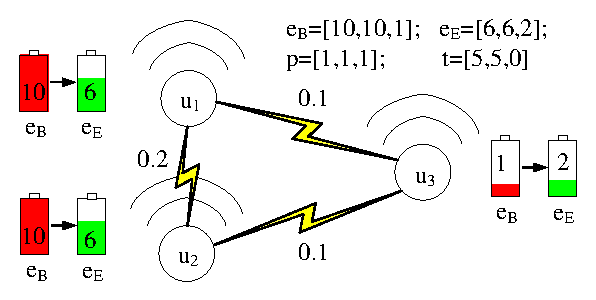
\includegraphics[width=0.38\textwidth]{fig3_2full.eps}}
\caption{An example without practical schedules assuring energy optimality of the WPTERD-Egy problem's solution.}
\label{fig_full}
\end{figure}

\vspace{-4mm}
\begin{figure}[htb]
\centering{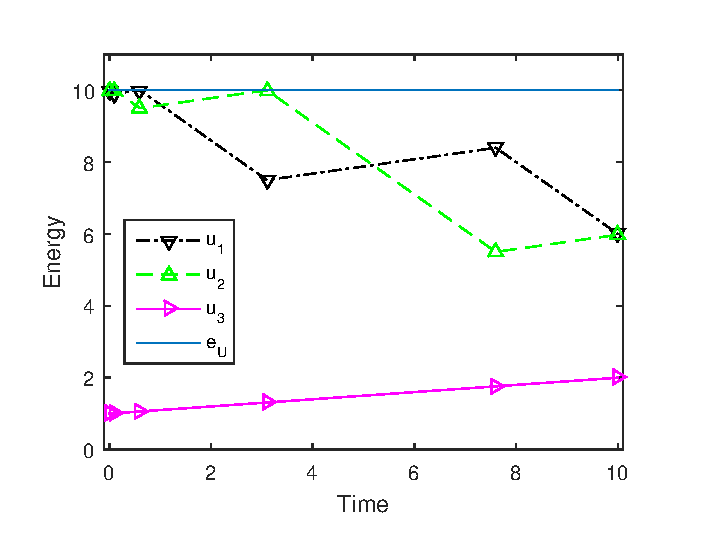
\includegraphics[width=0.42\textwidth]{fig4_2full_sch.eps}}
\caption{The energy changing processes of the nodes along with time of a schedule for the example in Fig.\ref{fig_full}.}
\label{fig_full_sch}
\end{figure}

\subsection{Performance Ratios of the LNSWL-SS Algorithm}
The rough superiority of the solutions returned by an approximate algorithm is usually implied by its performance ratio. Performance ratio of an algorithm is a constant $\rho{\geq}1$ such that, for any instance $I$ of the maximization(minimization) problem, the value of any solution returned by the algorithm is at least $1/{\rho}$ (at most $\rho$ times of) of the optimal value. A polynomial time approximation scheme (PTAS) for a problem is a polynomial time approximation algorithm which guarantees performance ratio of $1{+}\epsilon$ for some $\epsilon{>}0$.

For general graphs, the graph coloring problem is NP-hard even for any fixed number of colors $k{\geq}3$~\cite{Garey1979}. Furthermore, it is hard to approximate, \text{i.e.}, the problem of approximating the chromatic number with any constant ratio is also NP-hard~\cite{Arora1992}. Fortunately, for the ETTS problems embedded in the WPTERD-Time problem, the conflict graphs are intersection graphs of the nodes' energy signal coverage disks, we find that our LNSWL-SS Algorithm has constant approximations.

\begin{lemma}
\label{lemma_valid_solution}
The LNSWL-SS Algorithm can definitely find a solution to the ETTS problem with makespan not greater than $\varpi(G)$, \textit{i.e.,} all time slices fall in time interval $[0,\varpi(G)]$.
\end{lemma}

\begin{IEEEproof}
We will prove it by induction. The LNSWL-SS algorithm determines the time slices of the nodes in the sequence of $v_\text{List}[1{:}n]$. For the first node $v_\text{List}(1)$, it is obvious that its energy transmission operation can definitely be scheduled in time interval $[0,\varpi(G)]$. Now assume that the time slices for the nodes in $v_\text{List}[1{:}i]$ are in $[0,\varpi(G)]$. According to the definition of $\varpi(G)$ and the construction of the list $v_\text{List}[1{:}n]$, we must have $w(N(v_\text{List}(i{+}1))){\leq}\varpi(G)$, otherwise we will have $\varpi(G){\geq}w(N(v_\text{List}(i{+}1)))$ according to the way $\varpi(G)$ is updated by code line~\ref{v_update}. Hence, we can surely schedule node $v_\text{List}(i{+}1)$'s energy transmission operations in between the time slices occupied by its neighbors meanwhile kept in interval $[0,\varpi(G)]$. The lemma follows.
\end{IEEEproof}

\begin{lemma}
\label{lemma_2d_ratio3}
For WSNs in 2D space, if the nodes' energy coverage disks have equal radii, then the LNSWL-SS Algorithm has an approximation ratio of 3.
\end{lemma}

\begin{IEEEproof}
Our proof mimics the proof of the theorem in []. First, the makespan $m_\text{OPT}$ of any optimal schedule must not be smaller than the weight of the maximum clique $w_\text{c,G}$, we have Eq.\eqref{eqn_pr_2d3_1}.

\begin{equation}
\label{eqn_pr_2d3_1}
m_\text{OPT}{\geq}w_\text{c,G}
\end{equation}

We let $H$ be a subgraph of $G$ such that every node in $H$ has neighbor-set-weight at least $\varpi(G)$, and let $v^{*}{\in}H$ be the node having smallest $Y$. Using the definition of $\varpi(G)$ and Lemma \ref{lemma_valid_solution}, we have Eq.\eqref{eqn_pr_2d3_2}.

\begin{equation}
\label{eqn_pr_2d3_2}
w_\text{N,y}(v^{*},H){\geq}\varpi(G){\geq}m_\text{LNSWL}
\end{equation}

Since that $v^{*}$ has the smallest $Y$ coordinate in $H$, all nodes in $H$ must be in the top half plane above the horizontal line through node $v^{*}$. We divide the right half disk with radius $r$ into three equal sections as shown in Fig.\ref{fig_2d3part}, where nodes represented by blue circles are the nodes in $N(v^{*},H){=}H{\cap}N(v^{*})$. Nodes on the division lines can be assumed to be in either of the two adjacent sections deterministically.

\begin{figure}[htb]
\centering{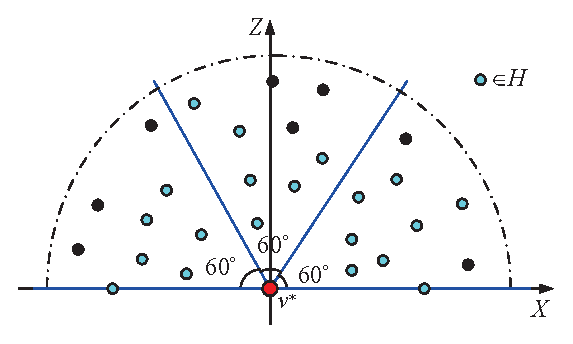
\includegraphics[width=0.35\textwidth]{fig_2d3part.eps}}
\caption{Divide the top half disk into 3 sections.}
\label{fig_2d3part}
\end{figure}

Since that all the nodes have energy signal radius $r$, it is obvious that the nodes in each section form a clique. Assume the maximum weight clique of the graph $G$ has weight $w_\text{c,G}$, then we have Eq.\eqref{eqn_pr_2d3_3}.

\begin{equation}
\label{eqn_pr_2d3_3}
\begin{array}{rcl}
w_\text{N,y}(v^{*},H)&{=}&w(S_1{\cap}H{+}S_2{\cap}H{+}S_3{\cap}H{-}2{*}w(v^{*}))\\
&{\leq}&w(S_1{\cap}H{+}S_2{\cap}H{+}S_3{\cap}H){\leq}3\\
&{\leq}&3{*}w_\text{c,G}
\end{array}
\end{equation}

Combining the equations from Eq.\eqref{eqn_pr_2d3_1} to Eq.\eqref{eqn_pr_2d3_3}, we obtain $m_\text{LNSWL}{\leq}3{*}m_\text{OPT}$. The lemma follows.
\end{IEEEproof}


\begin{lemma}
\label{lemma_3d_ratio12}
For WSNs in 3D space, if the nodes' energy coverage spheres have equal radii, then the LNSWL-SS Algorithm has an approximation ratio of 12.
\end{lemma}

\begin{IEEEproof}
The proof process is identical to that used in the previous lemma, but with some adaptations to the 3D space. The differences lie in the following aspects. (1) $v^{*}$ represents the node with smallest $Z$ coordinate value in $H$; (2) divide the top half sphere into 12 sections as shown in Fig.\ref{fig_3d12part} (firstly use the planes $X{=}0$ and $Y{=}0$ to split the half sphere into 4 equal sections, then divide each section into 3 sections using three planes, each of which contains the line through point (0,0,0) and the center point of the section's spherical face meanwhile perpendicular to the partition planes).

\begin{figure}[htb]
\centering{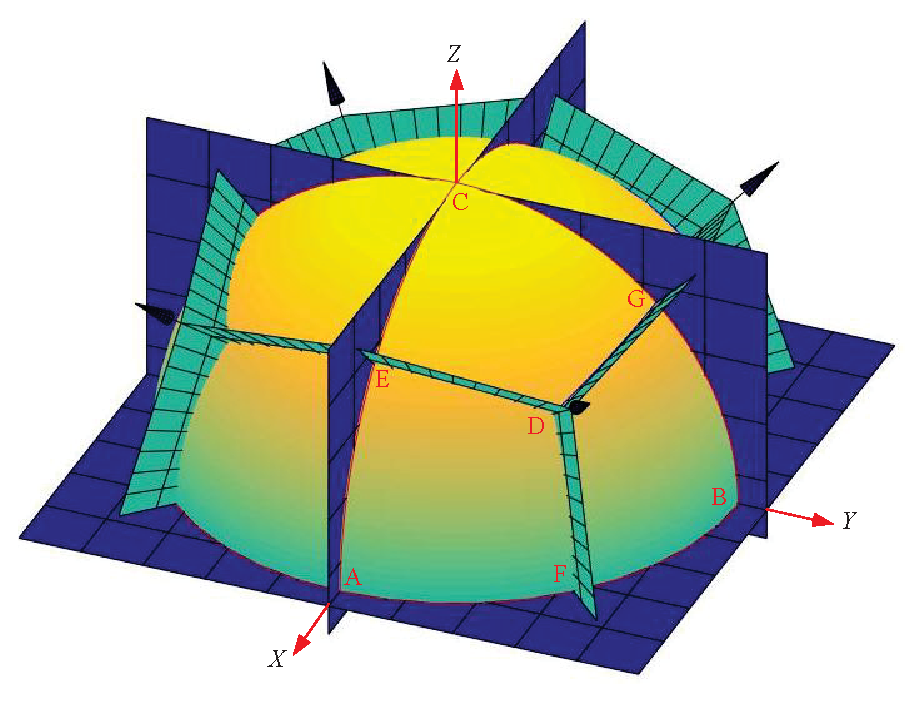
\includegraphics[width=0.35\textwidth]{fig_3d12part.eps}}
\caption{Divide the top half sphere into 12 sections.}
\label{fig_3d12part}
\end{figure}

It is easy to notice that any two points in one section has distance not greater than coverage radius $r$. For example, the distances between the points $A$, $D$, $E$, $F$ in the same section in Fig.\ref{fig_3d12part} can be obtained easily as $l_{DA}{=}r{*}\sqrt{(1{-}1/\sqrt{3})^2{+}2*(1/\sqrt{3})^2}{\approx}0.9194r{<}r$, $l_{DE}{=}l_{DF}{=}r{*}\sqrt{2(1/\sqrt{2}{-}1/\sqrt{3})^2{+}(1/\sqrt{3})^2}{\approx}0.6058r{<}r$, $l_{EF}{=}r{*}\sqrt{2{*}(1/\sqrt{2})^2}{=}r$. Thus, all nodes in each section must form a clique.

Applying the analysis process to the 3D case with above adaptations, we obtain $m_\text{LNSWL}{\leq}12{*}m_\text{OPT}$. The lemma follows.
\end{IEEEproof}

For the general case of the nodes' energy transmission signals having different coverage radius, we have the following lemma about performance ratio of LNSWL-SS.

\begin{lemma}
\label{lemma_2d3d_ratio}
For WSNs in 2D (3D) space, if the radius of the nodes' energy coverage disks (spheres) do not equal, then the LNSWL-SS Algorithm has an approximation ratio of 6 (24).
\end{lemma}

\begin{IEEEproof}
These can be proved by applying an analysis method similar to that used in proving the previous lemmas, but with some adaptations to the non-equal radii condition. To be specific, assume $H$ is a subgraph of $G$ such that every node in $H$ has neighbor-set-weight at least $\varpi(G)$, we select $v^{*}{\in}H$ be the node having smallest radius $r_1$. Thus, all other nodes in $H$ may lie around the node $v^{*}$, instead of lie in a half space of $v^{*}$. Hence, for assuring that all nodes in a section form a clique, for the 2D case, we have to divide the disk centered at $v^{*}$ with radius $r_1$ into 6 equal sections as shown in Fig.\ref{fig_2d6part}.

\begin{figure}[htb]
\centering{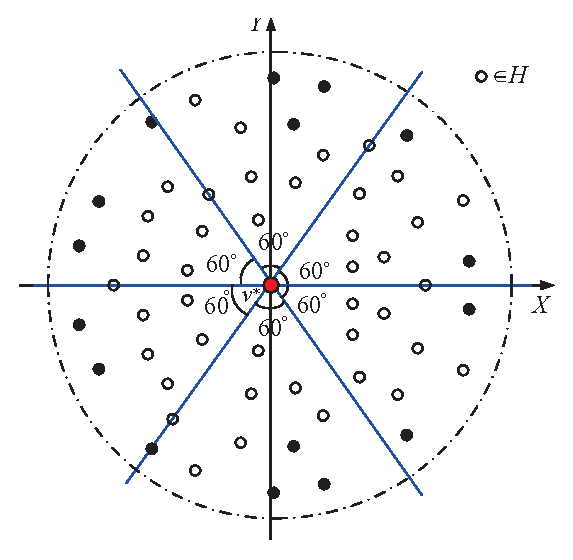
\includegraphics[width=0.35\textwidth]{fig_2d6part.eps}}
\caption{Divide the disk centered at $v_{*}$ with radius $r_1$ in 2D space into 6 sections.}
\label{fig_2d6part}
\end{figure}

For the 3D case, we have to divide the sphere centered at $v^{*}$ with radius $r_1$ into 24 equal sections as shown in Fig.\ref{fig_3d24part}.

\begin{figure}[htb]
\centering{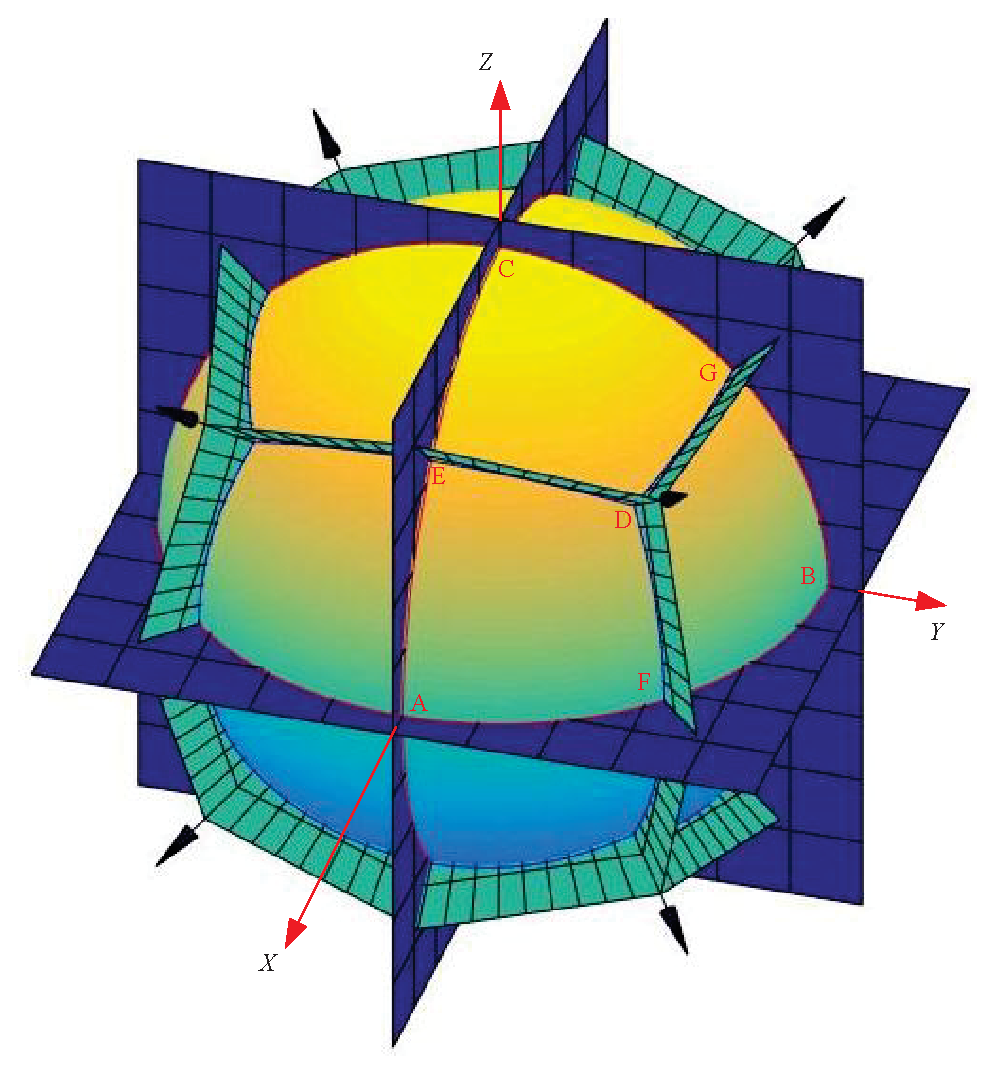
\includegraphics[width=0.35\textwidth]{fig_3d24part.eps}}
\caption{Divide the sphere centered at $v_{*}$ with radius $r_1$ in 3D space into 24 sections.}
\label{fig_3d24part}
\end{figure}

Further analyses will correspondingly result to performance ratio of 6 and 24, respectively. The lemma follows.

\end{IEEEproof}

\section{Solve the WPTERD Problem}

Based on previous analyses results and the preliminary algorithms proposed, we can thus solve the WPTERD problem by decoupling the problem into WPTERD-Egy problem and WPTERD-Time problem. The two problems focus exclusively on the optimization in energy and time, respectively. Based on this approach, we propose our algorithm named Energy Time Decoupling (ETDeCouple) algorithm. ETDeCouple firstly solve the \textbf{P3} problem using mature LP optimization softwares to obtain $\mathbf{t}$. Then, it obtains $S_\text{cts}$ by using the LNSWL-S algorithm to solve the corresponding ETTS problem, and at last generates a schedule $TS_\text{ss}$ from $S_\text{cts}$ by using the ETCS-S algorithm. The pseudo code of ETDeCouple is shown in Alg.\ref{Alg_ETDeCouple}.
 
\begin{algorithm}[!htb]
\caption{The ETDeCouple algorithm}
\begin{algorithmic}[1]\label{Alg_ETDeCouple}
    \REQUIRE $\mathbf{e_B}, \mathbf{e_U}, \mathbf{e_L}, \mathbf{e_E}, \mathbf{C}, \mathbf{p}$;\\
    \ENSURE $TS_\text{ss}$: the time-set schedule sequence;\\
    \STATE $[\mathbf{t}]${=}solveP3($\mathbf{e_B}, \mathbf{e_O},\mathbf{e_U},\mathbf{C}, \mathbf{p}$);\%using  to solve and obtain $\mathbf{t}$;\\
    \STATE create $G(V,E,W)$ for the corresponding ETTS problem using $\mathbf{t}$;
    \STATE $[S_\text{cts}]{=}$LNSWL-SS$(G(V,E,W)$;
    \STATE $[TS_\text{ss}]{=}$ETCS-S$(S_\text{cts},\mathbf{e_B}, \mathbf{e_U}, \mathbf{e_L}, \mathbf{e_E}, \mathbf{C}, \mathbf{p})$;
     \STATE \textbf{return} $TS_\text{ss}$;
\end{algorithmic}
\end{algorithm}

\textit{By using the ETDeCouple algorithm to carefully schedule the energy transmissions of the nodes in WSNs, we are able redistribute energy in the network, which implicitly realizes the multi-hop energy flow efficiently but easily. Meanwhile, the broadcasting nature of radio signals is well exploited to achieve the most energy efficient way to conduct the energy redistribution}.

\section{Performance Evaluation}
\label{sec_sim}
\subsection{Performance Metrics}
We conduct numerical simulations using Matlab 2015a on a computer with Win10-bit64, 2.21GHz i7-CPU, and 8GB Memory. Three performance metrics are used: \textit{Energy Loss Ratio}, \textit{Schedule Makespan}, and \textit{Switch Number}. The energy loss ratio metric is calculated as  $\frac{\sum_{i{\in}\mathcal{N}(n)}(e_\text{B}(i){-}e_\text{F}(i))}{\sum_{i{\in}\mathcal{N}(n),e_\text{E}(i){>}e_\text{B}(i)}(e_\text{E}(i){-}e_\text{B}(i))}$   , which implies the side 'cost' for redistribute energy in the network using the algorithm. The makespan metric represents the the time span of the energy transmissions of a schedule, which reveals the time efficiency of a schedule. The switch number metric represents the number of energy transmissions slices of the nodes in the schedule, which is obtained by counting the starts of energy transmissions. This metric implies the number of node status changes in a schedule. We obviously prefer smaller energy loss, smaller schedule makespan, and smaller switch number.

\subsection{Simulation Setup}
We test our GERDS algorithm with two node selection policies: (1) select the node with maximum $t$, (2) select the node whose energy is most close to $e_\text{U}$(i.e., to select the node with maximum energy if all nodes have the same $e_\text{U}$. We denote them as GERDS-MaxT and GERDS-MaxEgy, respectively. For comparison purpose, we implement another algorithm denoted as AlgNoParallel, where the nodes transmit energy one by one without parallel, even for not-neighboring nodes. In AlgNoParallel, the time for each continuous energy transmission slice is determined in a way similar to that in GERDS. Additionally, it is obvious that the maximum clique of the weighted graph $G(V,E,W)$ of the WPTERD-Time problem  is a lower bound for the makespan of an optimal schedule. We use a greedy-based algorithm denoted as LBClique to approximately solve the maximum weight clique problem and use it as a baseline for performance evaluation. Thus, totaly four algorithms are tested in our simulations: GERDS-MaxT, GERDS-MaxEgy, AlgNoParallel, LBClique.

Main parameters and the default values in our simulations include \textit{number of nodes} $n{=}100$, \textit{side length} $L{=}10$ of the square network region, \textit{energy transmission power} $p{=}1$, \textit{ratio of energy-needing nodes} $\eta{=}0.3$, and \textit{the amount of energy required by these energy-needing nodes} $e_\text{h}{=}5$, $e_\text{U}{=}100$, $e_\text{L}{=}20$. The energy harvesting coefficients are set as $\alpha{=}0.3$, $\beta{=}1$, $\gamma{=}2$, and $D{=}4$,. A set of particular values for these parameters is called a \textbf{simulation configuration}. For each simulation configuration, 100 problem instances are generated and treated using the tested algorithms in turn. The WPTERD-Egy problem of randomly generated WSNs may have no LP solutions at all, in such cases new problem instances are generated repeatedly until a valid problem instance is obtained. In each problem instance, $n$ nodes are randomly placed in the square region $L{\times}L$ (Although our analysis applies to 3D space, we restrict our simulations for 2D case without sacrificing the effectiveness of the simulation results). $e_\text{B}(i)$, $i{\in}\mathcal{N}(n)$, are randomly selected in $[e_\text{L},e_\text{U})$ following the uniform distribution. Randomly select ${\lceil}n{*}\eta{\rceil}$ energy-needing nodes and set $e_\text{E}(i)$ of each node $u_i$ in this set to be $e_\text{E}(i){+}e_\text{h}$. All the others nodes' energy expectations are set to $e_\text{L}$. Results of the performance metrics are collected and averaged to obtain the final results for the simulation configurations. The 95\% confidence intervals of the performance metrics are also calculated.

\subsection{Simulation Results}

In our simulation experiments, the effects of a parameter on the algorithms' performance are obtained by performing a simulation set consisting of similar simulation configurations. The simulation configurations in such simulation set only difference in the value of this parameter, whereas all the other parameters take their default values. We conduct simulation experiments for inspecting the effects of the main parameters. All simulation results verify the efficiency of our algorithms. Here we only provide the simulation results for parameter $n$ for space limitation.

In the simulation experiment for $n$, we let $n$ take values in range from 10 to 100 with step size 10. The results are shown in Fig.\ref{fig_sim_n}. The energy loss ratio switch number metric is not applicable to LBClique. Since that the other three algorithms make schedules based the shared solution $t$ of \textbf{P3}, there are no distinctive differences in the energy loss ratio metric, as shown in Fig.\ref{fig_sim_n}(a). As $n$ increases, the energy loss ratio decreases quickly. This is reasonable since that, with higher node density, the energy harvesting coefficients will be much larger, and more nodes can harvest energy from the single energy transmission. These two factors both lead to less energy loss when transmitting energy to others. The results in Fig.\ref{fig_sim_n}(b) show that, GERDS-MaxT and GERDS-MaxEgy obtain similar makespans, which are both no more than 120\% of LBClique. These results imply that GERDS-MaxT and GERDS-MaxEgy are nearly optimal. Compared with AlgNoParallel, GERDS-MaxT and GERDS-MaxEgy reduces the makespan metric by more than 60\% when $n{=}100$, and the it will become more effective in this metric as $n$ increases. These results impliy that the GERDS based algorithms can exploit the parallel energy transmitting opportunities well. This is obtained at the cost of a little more operation status switches, as shown in Fig.\ref{fig_sim_n}(c).
GERDS-MaxEgy outperforms GERDS-MaxT in this metric. Compared with AlgNoParallel, when $n{=}100$, GERDS-MaxEgy incurs only about 5\% more switches, whereas it is about 20\% for GERDS-MaxT.

\begin{figure*}[!htbp]
\centering{
\begin{minipage}[c]{0.30\textwidth}
\centering{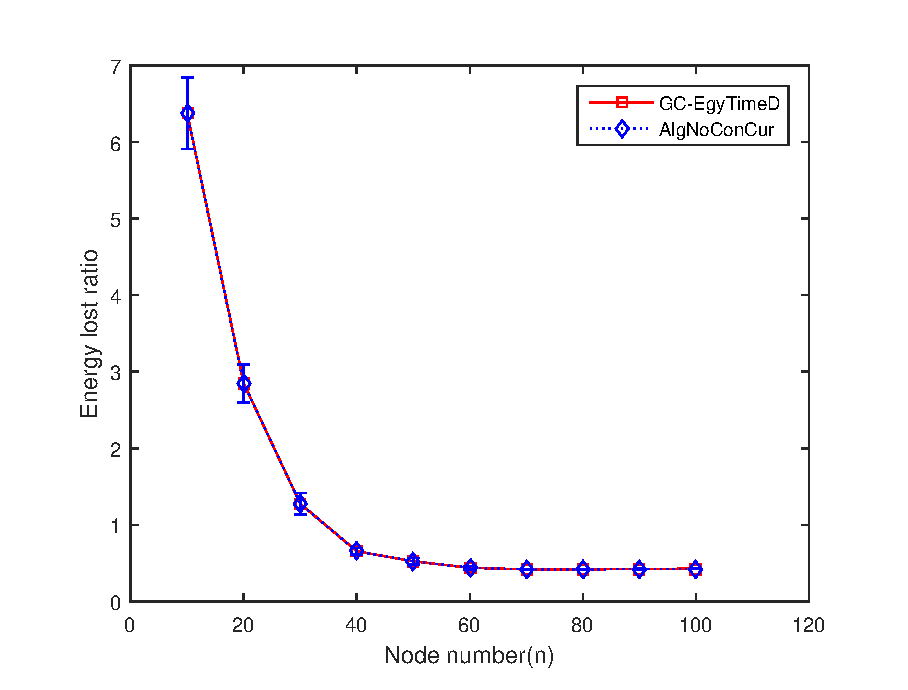
\includegraphics[width=\textwidth]{sim_n100_egy.eps}}
\parbox{\linewidth}{\centering\small{(a)energy loss ratio}}
\end{minipage}%
\hspace{0.01\textwidth}%
\begin{minipage}[c]{0.30\textwidth}
\centering{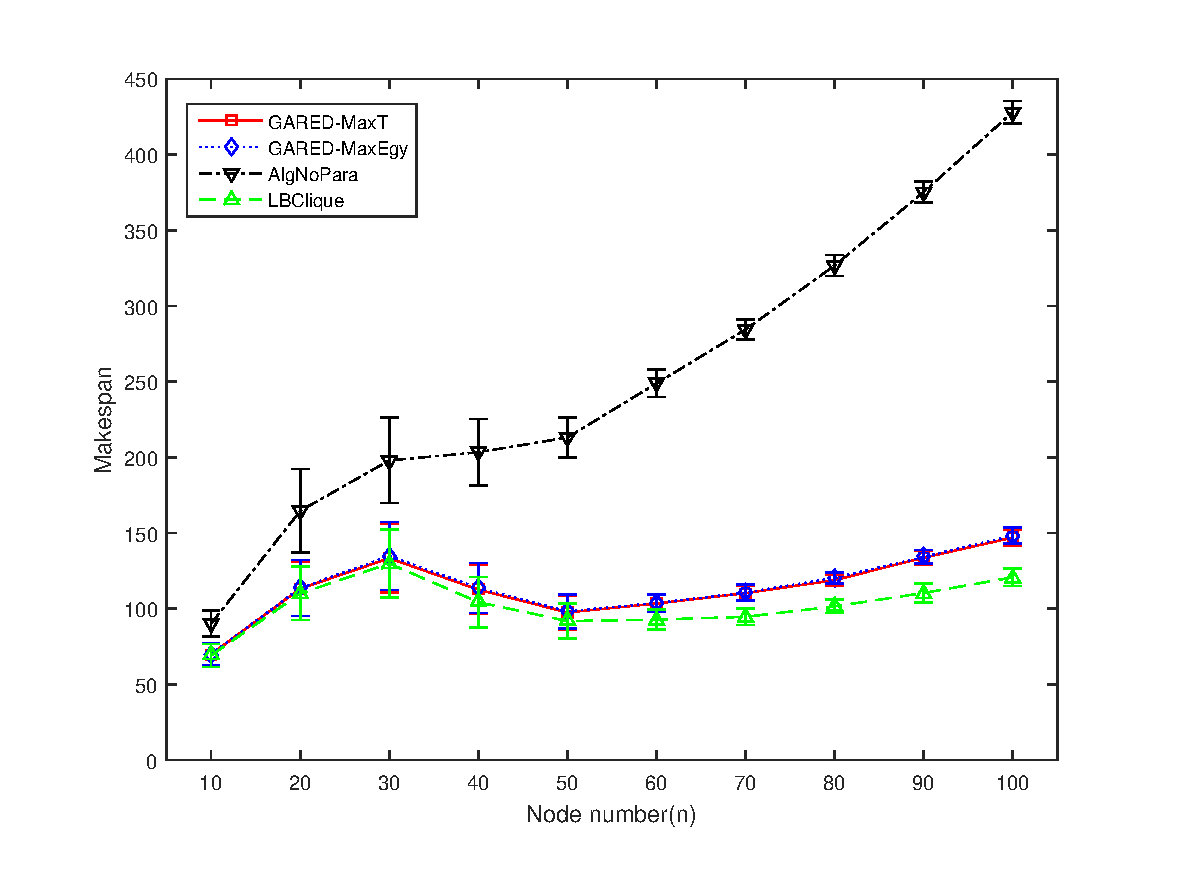
\includegraphics[width=\textwidth]{sim_n100_makespan.eps}}
\parbox{\linewidth}{\centering\small{(b)makespan}}
\end{minipage}
\hspace{0.01\textwidth}%
\begin{minipage}[c]{0.30\textwidth}
\centering{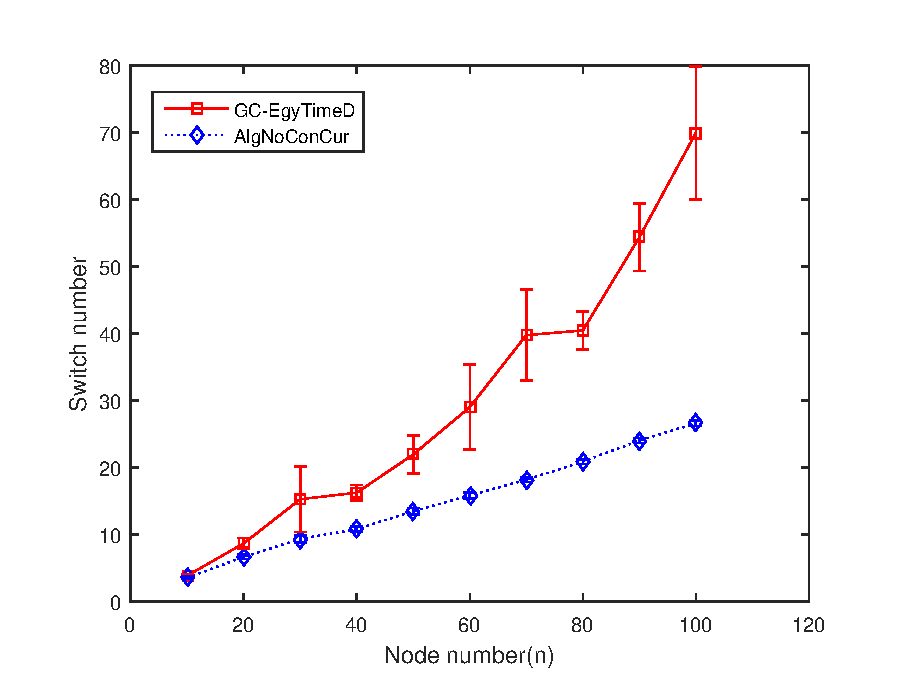
\includegraphics[width=\textwidth]{sim_n100_switchnum.eps}}
\parbox{\linewidth}{\centering\small{(c)switch number}}
\end{minipage}
}
\caption{The effect of node number $n$ on performance of the algorithms.}
\label{fig_sim_n}
\end{figure*}


\section{Conclusion}
\label{sec_conclusion}
In this paper, we propose a two-step approach to solve the WPTERD problem by solving two embedded sub-problems WPTERD-Egy and WPTERD-Time in turn. In the first step, by formulating the WPTERD-Egy problem based on interesting property of the problem in a linear programming (LP) form, we obtain the optimal energy transmitting time lengths of the nodes leading to minimum energy loss. With the results in the first step, the remanent work of the WPTERD problem becomes the WPTERD-Time problem, which is to find a minimum makespan schedule not violating the nodes' energy limits. We prove that the WPTERD-Time problem is NP-hard, and then we propose a greedy-based heuristic algorithm named GERDS to solve it. Numerical simulations illustrate the effectiveness and efficiency of GERDS, which return schedules with minimum energy loss and approximately minimum makespan. By exploiting parallel opportunities of energy transmissions, GERDS reduces makespan by more than 60\% when compared with a schedule without exploiting the parallel energy transmission opportunities.


% use section* for acknowledgement
\section*{Acknowledgment}
This research was funded by Natural Science Foundation of China (No.XXXXXXXX, XXXXXXXX, XXXXXXXX).

\ifCLASSOPTIONcaptionsoff
  \newpage
\fi


\begin{thebibliography}{11}
% You can use other form of bib file by changing here...

\bibitem{Kurs2007}
A. Kurs, A. Karalis, R. Moffatt, J. D. Joannopoulos, P. Fisher, and M. Soljacic, "Wireless power transfer via strongly coupled magnetic resonances", \textit{Science}, vol.317, no.5834, pp.83-86, 2007.

\bibitem{Cannon2009}
B. Cannon, J. Hoburg, D. Stancil, and S. Goldstein, "Magnetic resonant coupling as a potential means for wireless power transfer to multiple small receivers", \textit{IEEE Transactions on Power Electronics}, vol.24, no.7, pp.1819-1825, July 2009.

\bibitem{Kang2006}
K. Kang, Y. S. Meng, J. Breger, C. P. Grey, and G. Ceder, "Electrodes with high power and high capacity for rechargeable lithium batteries", \textit{Science}, vol.311, no.5763, pp. 977-980, 2006.

\bibitem{Guo2017}
P. Guo, X. F. Liu, S. J. Tang, J. N. Cao, "Concurrently wireless charging sensor networks with efficient scheduling," \textit{IEEE Transactions on Mobile Computing}, vol.16, No.9, pp.2450-2463, Sep. 2017.

\bibitem{Nintana2012}
P. Nintanavongsa, U. Muncuk, D. R. Lewis, and K. R. Chowdhury, "Design optimization and implementation for RF energy harvesting circuits," \textit{IEEE Journal on Emerging and Selected Topics in Circuits and Systems}, vol.2, no.1, pp.24-33, 2012.

\bibitem{Xiang2013}
L. Xiang, J. Luo, K. Han, and G. T. Shi, "Fueling wireless networks perpetually: a case of multi-hop wireless power distribution," in \textit{Proc. IEEE 24th Annual International Symposium on Personal, Indoor, and Mobile Radio Communications (PIMRC2013)}, London, UK, 8-11 Sep. 2013, pp.1994-1999.

\bibitem{Rault2013}
T. Rault, A. Bouabdallah, Y. Challal, "Multi-hop wireless charging optimization in low-power networks," IEEE Global Communications Conference, 2013, Atlanta, United States. pp.484-489, 2013.

\bibitem{Guo2016}
P. Guo, X. F. Liu, T. F. Tang, S. J. Tang, J. N. Cao, "Practical concurrent wireless charging scheduling for sensor networks," in \textit{Proc. IEEE 36th International Conference on Distributed Computing Systems(ICDCS2016)}, Nara, Japan, 27-30 Jun. 2016, pp.741-742.

\bibitem{Bulut2014}
E. Bulut, M. E. Ahsen, B. K. Szymanski, "Opportunistic wireless charging for mobile social and sensor networks", in \textit{Proc. IEEE 6th International Workshop on Management of Emerging Networks and Services(Globecom2014)}, Austin, TX, USA, 8-12 Dec. 2014, pp.207-212.

\bibitem{Niko2016}
S. Nikoletseas, T. P. Raptis, C. Raptopoulos, "Energy balance with peer-to-peer wireless charging," in \textit{Proc. IEEE 13th International Conference on Mobile Ad Hoc and Sensor Systems(MASS2016)}, Brasilia, Brazil, 10-13 Oct. 2016, pp.101-108.

\bibitem{Niko2017}
S. Nikoletseas, T. P. Raptis, C. Raptopoulos, "Wireless charging for weighted energy balance in populations of mobile peers," \textit{Ad Hoc Networks}, vol.60, pp.1-10, 2017.

\bibitem{Madhja2016}
A. Madhja, S. Nikoletseas, C. Raptopoulos, "Energy aware network formation in peer-to-peer wireless power transfer," in \textit{Proc. ACM 19th International Conference on Modeling, Analysis and Simulation of Wireless and Mobile Systems (MSWiM2016)}, Malta, Nov. 13-17, 2016, pp.43-50.

\bibitem{Madhja2017}
A. Madhja, S. Nikoletseas, T. P. Raptis, C. Raptopoulos, and D. Tsolovos, "Peer-to-peer wireless energy transfer in populations of very weak mobile nodes," in \textit{Proc. IEEE Wireless Communications and Networking Conference Workshops (WCNCW2017)}, San Francisco, CA, USA, 19-22 Mar. 2017, pp.1-6.

\bibitem{Marx2004}
D$\acute{a}$niel Marx, "Graph colouring problems and their applications in scheduling," \textit{Periodica Polytechnica SER. EL. ENG.}, vol. 48, no.1, pp.11-16, 2004.

\bibitem{He2013}
S. He, J. Chen, F. Jiang, D. K. Y. Yau, G. Xing, and Y. Sun, "Energy provisioning in wireless rechargeable sensor networks," \textit{IEEE Transactions on Mobile Computing}, vol.12, no.10, pp.1931-1942, Oct. 2013.

\bibitem{Dai2017TON}
H. P. Dai, Y. H. Liu, G. H. Chen, X. B. Wu, T. He ; A. X. Liu, H. Z. Ma, "Safe charging for wireless power transfer," \textit{IEEE/ACM Transactions on Networking}, vol.25, no.6, pp.3531-3544, Dec. 2017.

\bibitem{Dai2018TON}
H. P. Dai, H. Z. Ma, A. X. Liu, and G. H. Chen, "Radiation constrained scheduling of wireless charging tasks," \textit{IEEE/ACM Transactions on Networking}, vol.26, No.1, pp.314-326, Feb. 2018.

\bibitem{Garey1979}
M. R. Garey, and D. S. Johnson, "Computers and Intractability," \textit{A Guide to the Theory of NP-Completeness}, W. H. Freeman and Company, New York, 1979.

\bibitem{Arora1992}
S. Arora, C. Lund, R. Motwani, M. Sudan, and M. Szegedy, "Proof verification and the intractability of approximating problems," in \textit{Proc. 33rd Annual IEEE Symposium on the Foundations of Computer Science}, 1992.

\bibitem{Roberts1978}
F.S. Roberts, Graph Theory and its Applications to Problems of Society, SIAM, 1978.

\bibitem{Hale1980}
W.K. Hale, ��Frequency Assignment: Theory and Applications,�� Proc. IEEE, Vol. 68,
1980, pp 1497-1514.

\bibitem{Kammerlander1984}
K. Kammerlander, ��C 900 �C An Advanced Mobile Radio Telephone System with Optimum
Frequency Utilization,�� IEEE Trans. Selected Areas in Communication, Vol. 2,
1984, pp 589-597.

\bibitem{Yeh1984}
Y. Yeh, J. Wilson and S.C. Schwartz, ��Outage Probability in Mobile Telephony with Directive
Antennas and Macrodiversity,�� IEEE Trans. Selected Areas in Communication,
Vol. 2, 1984, pp 507-511.

\bibitem{Wong1988}
D.W. Wong and Y.S. Kuo, A Study of Two Geometric Location Problems, Inf. Proc.
Letters, Vol. 28, No. 6, Aug. 1988, pp 281-286.

\bibitem{Hochbaum1983}
D. S. Hochbaum, "Efficient Bounds for the Stable Set, Vertex Cover and Set Packing
Problems," \textit{Discrete Applied Mathematics}, no.6, 1983, pp.243-254.

\end{thebibliography}


%It is not necessary to upload the biography when you submit your manuscript.


\end{document}
